\chapter{Experimental Verification}
\label{chap:experiment}

Using the knowledge gained by the simulation, an experiment at the beamline 3 of the SACLA FEL was performed. The experiment consisted of three parts: First, reproducing the results of Nakumura et al. and imaging projection of the focal volume of the FEL by using metal foils as samples, performing a measurement of the K$_\alpha$  fluorescence and an reconstruction in the small angle regime \cite{nakumura2020}.  Second, moving to a smaller length scale and trying to image nanoparticles. And third, leaving the small angle regime and recording the fluorescence of a single crystal and perform a three dimensional reciprocal space reconstruction. 
%XXX Bekannte samples
%% different geometry

In this chapter, the sample preparation and characterization by small angle scattering at the SSRL synchrotron, electron microscopy and X-ray diffraction performed at the SLAC National Accelerator  Laboratory (US), the experimental setup at SACLA (Japan), the methods of data analysis and the results will be presented and finally discussed.

\section{Sample Preparation and Characterization}
As a nanoparticle sample, spherical iron oxide  (magnetite) nanoparticles were chosen for their commercial availability in high quality. For the sample delivery method, deposition in polymer matrices was chosen to simplify finding the spatial overlap between the FEL beam and the sample (compared to for example injectors) and to require little changes in the setup to switch between the metal foils and the nanoparticle sample. 
Galliumarsnide (GaAS) was chosen as a crystalline sample for its comparatively simple structure and large product its lattice constant and the gallium K${_\alpha}$ fluorescence energy, resulting in lower scattering angles necessary to record the Bragg peaks compared to other commonly used single crystals. 

\subsection{Magnetite Nanoparticle in Polymer Samples}
To allow (statistically) multiple particles inside the focus to improve the number of detected fluorescence photons per FEL shot and greatly reduced the possibility of having shots without any particles inside the focus as well, the following preparation was developed:

Magnetite nanoparticles coated with oleic acid and dispersed in toluene were bought from NN-Labs (nominal diameters 5\,nm, 10\,nm and 20\,nm), inhibited methylmethacrylate (MMA) and etyhlhexylmethacrylate (EHMA)  (both Sigma Aldrich) were filtered using a prefilled column to remove the inhibitor,  2,2-azo-bis-isobutyrylnitrile (AIBN, Sigma Aldrich) was used as thermally activated radical initiator as received. Polystyrene (Sigma Aldrich, MW ~192k) and ferric chloride (97\%, Sigma Aldrich) was used as received. As solvents, methanol, toluene and chloroform were used.
\paragraph{Nanoparticles in Polystyrene Matrix} 
The nanoparticles were precipitated with methanol, centrifuged and redispersed in chloroform at a concentration of 25\,mg/ml (with the weight of nanoparticles including the weight of the oleic acid capping). Polystyrene was dissolved in chloroform at a concentration of 250\,mg/ml. 
To each of 700\,\textmu l solution of 5\,nm nanoparticles, 500\,\textmu l solution of 10\,nm nanoparticles and 425\,\textmu l solution of 20\,nm nanoparticles, respectively, 5\,ml of the polystyrene solution were added, approximatly accounting for the different iron concentration in the solutions.  After ensuring dispersion by strong sonication, fractions of 100\,\textmu l the solution were carefully dropped onto slowly spinning (100\,rpm for 5\,min) glass cover slips (20\,mm x 20\,mm). After drying, the approximately 200\,\textmu m thick films were removed from the glass slides.

As a control sample with approximately equal iron concentration, 60\,mg FeCl3 and 25\,g polystyrene were dissolved in 10\,ml acetone, sonicated and  fractions of 100\,\textmu l were dropped onto slowly spinning glass slides  and carefully removed after drying.
%\begin{table}[tp]
%	\centering
%	\caption{Nanoparticles in polystyrene recipes}
%	\label{tab:samplePS}
%	\begin{tabular}{llll}
%		\hline
%	NP size&   Volume NP in CF  &Volume PS in CF    \\
%		\hline
%	  5\,nm&700 ul & & 5\,ml  \\  
%	   10\,nm&  500 ul& &5\,ml  \\    
%	   20\,nm &  425 ul& &5\,ml  \\  
%	   	Control   &  & &5\,ml  \\  
%		\hline
%	\end{tabular}
%\end{table}

\paragraph{Nanoparticles in Poly-(methyl methacrylate / etylhexyl methacrylate)  Matrix}
As a second nanoparticle in polymer sample, an azobisisobutyronitrile initiated methyl methacrylate (MMA)/etylhexyl methacrylate (EHMA) polymerization with magnetite nanoparticles was performed. 
The nanoparticle solutions as bought were concentrated to 25\,mg/ml in toluene by precipitation with methanol, centrifugation and redispersion.  To varying amounts of the nanoparticle solution and additional toluene, 800\,\textmu l of EHMA was added each to account for the different iron concentrations (see \fref{tab:sampleCP}). After strong sonication to ensure dispersion, 3.2\,ml of MMA were added and the solution  bubbled with N$_2$ for 5\,min. To start the polymerization, 20\,mg of AIBN was added and the solution was bubbled again with N$_2$  for 10\,min before heating to 60°C under weak sonication using a sonic bath. The mixture was kept at temperature for 12h.
The vials were uncapped and the polymer dried for 12h at 50°C. The polymer was removed from the vials and cut into slices of approximately (150$\pm$20)\,\textmu m thickness using a slow spinning diamond saw.
As a control sample, the polymerization was performed without any nanoparticles added.

\begin{table}[tp]
	\centering
	\caption{Nanoparticles in PMMA/EHMA recipes}
	\label{tab:sampleCP}
	\begin{tabular}{llllll}
		\hline
		NP size &NP in Toluene&Toluene & EHMA & MMA & AIBN \\
		\hline
		5\,nm&1 \,ml & 0\,ml&0.8\,ml&  3.2\,ml&   20\,mg    \\
		10\,nm& 0.8\,ml& 0.2\,ml & 0.8\,ml&  3.2\,ml&   20\,mg    \\
		10\,nm& 0.8\,ml& 0,2\,ml &            &  4\,ml   &   20\,mg    \\
		20\,nm& 0.6\,ml& 0.4\,ml& 0.8\,ml&  3.2\,ml&   20\,mg    \\
		Control&           & 1\,ml     &800\,\textmu l&  3.2\,ml&   20\,mg    \\
		\hline
	\end{tabular}
\end{table}

\paragraph{Nanoparticle Sample Characterisation}
To characterize the nanoparticles before the embedding in a polymer, the iron oxide nanoparticles as received were diluted with toluene, deposited on a silicon nitride membrane and imaged using a FEI Tecnai microscope  (see \fref{fig:tem}).  For each of the three nominal sizes, 3 different areas on the membrane were analyzed using ImageJ, resulting in mean radii of 8.3$\pm$1.7\,nm (nominal \enquote{20\,nm} diameter), 4.1$\pm$0.8 \,nm	(\enquote{10\,nm} diameter) and 3.1$\pm$0.6\,nm (\enquote{5\,nm}), respectively. In the TEM images, the effect of the oleic acid ligands used to stabilize the nanoparticle dispersion can be seen as the inter-particle distance.

\begin{figure}[tp]
	\centering
	\begin{subfigure}[b]{0.25\textwidth}
		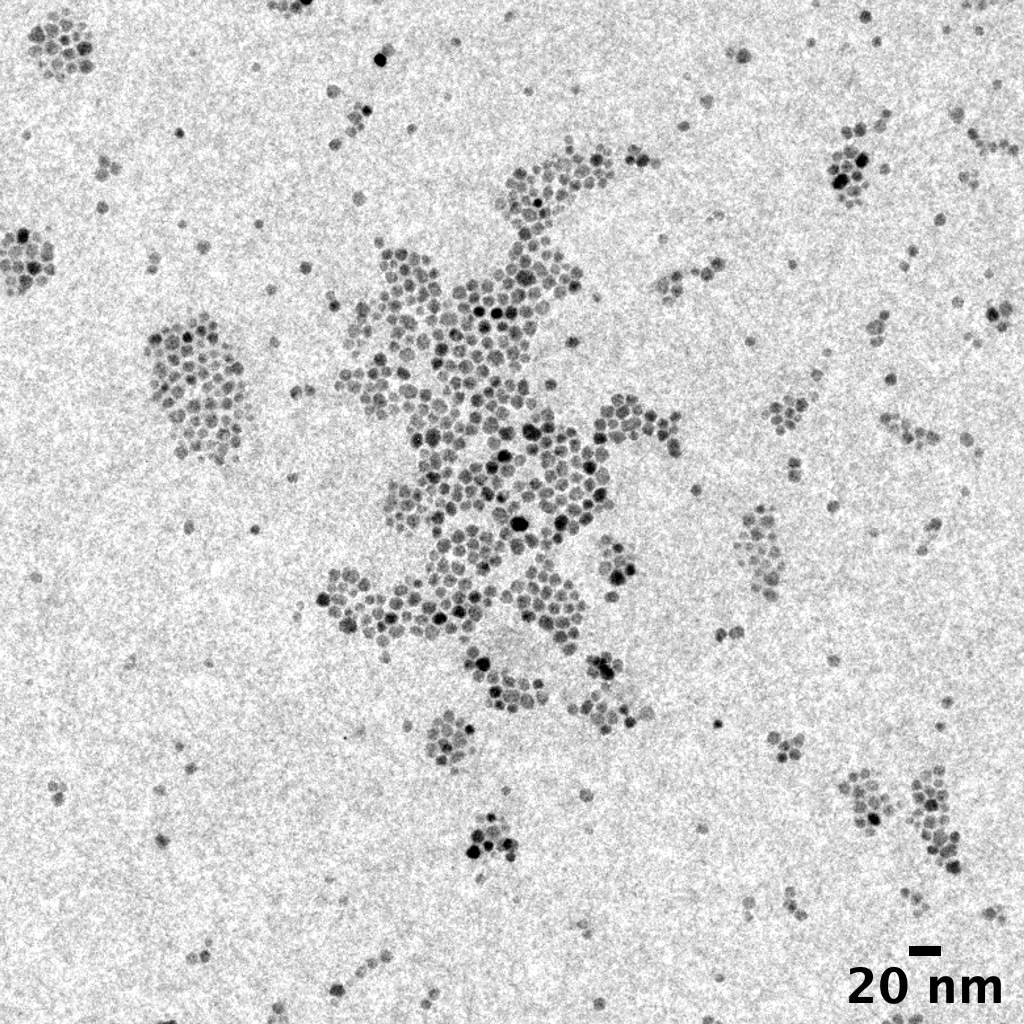
\includegraphics[width=\linewidth]{images/tem5.png}
	\end{subfigure}
	\begin{subfigure}[b]{0.25\textwidth}
		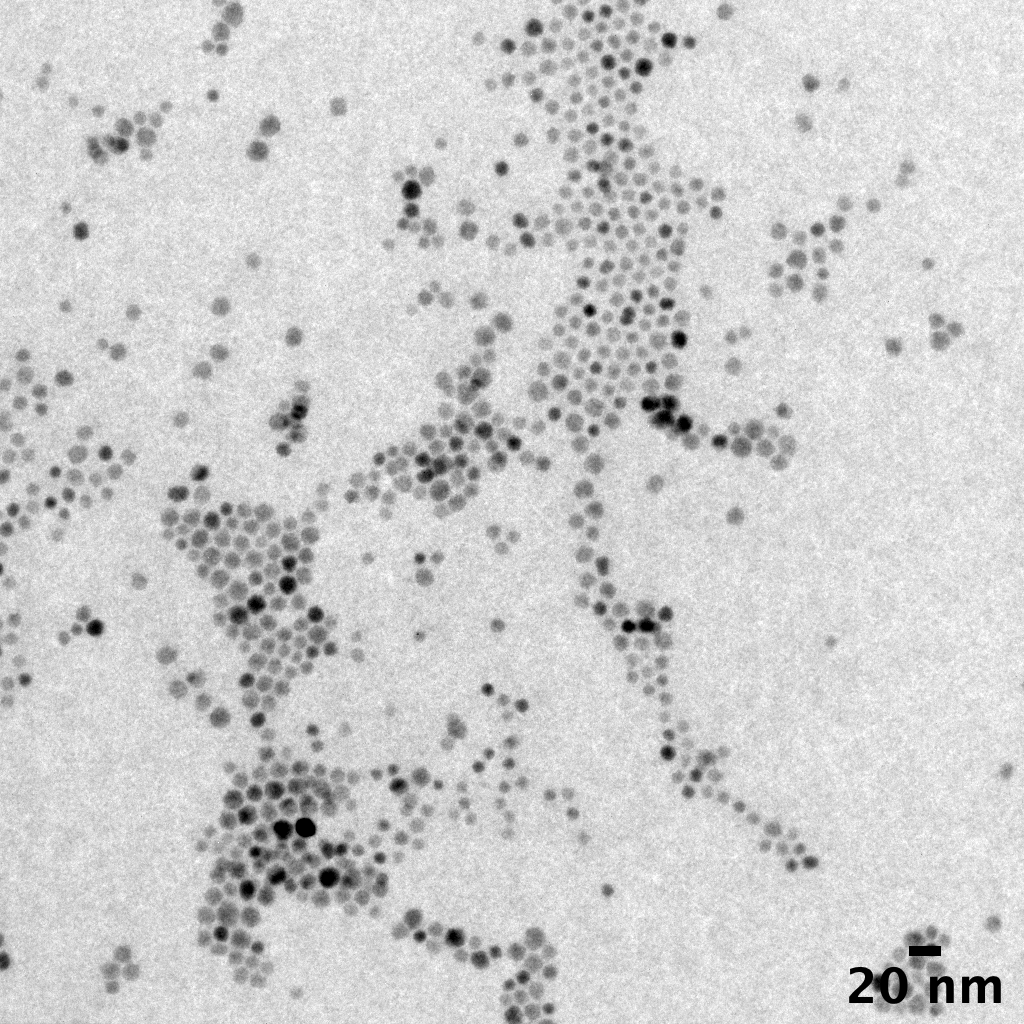
\includegraphics[width=\linewidth]{images/tem10.png}
	\end{subfigure}
	\begin{subfigure}[b]{0.25\textwidth}
		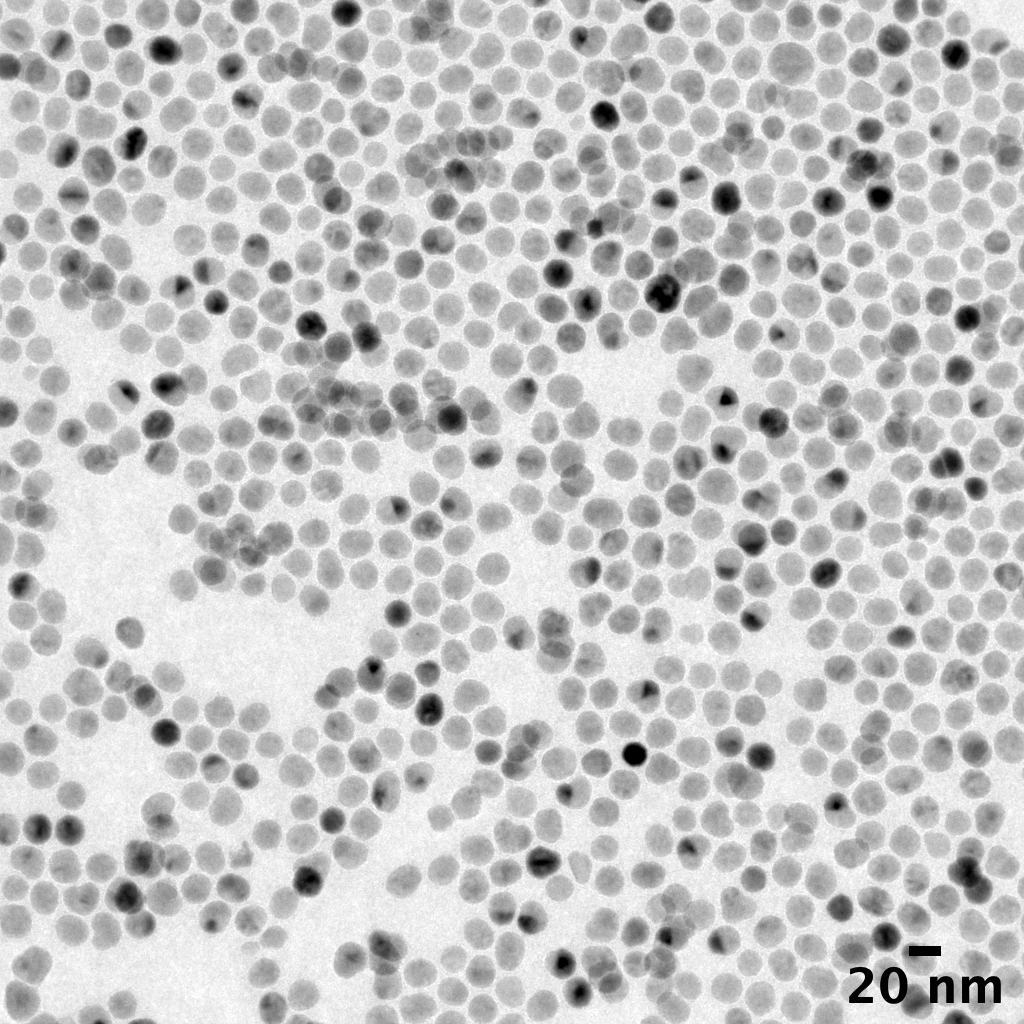
\includegraphics[width=\linewidth]{images/tem20.png}
	\end{subfigure}
\par\smallskip
	\begin{subfigure}[b]{0.25\textwidth}
		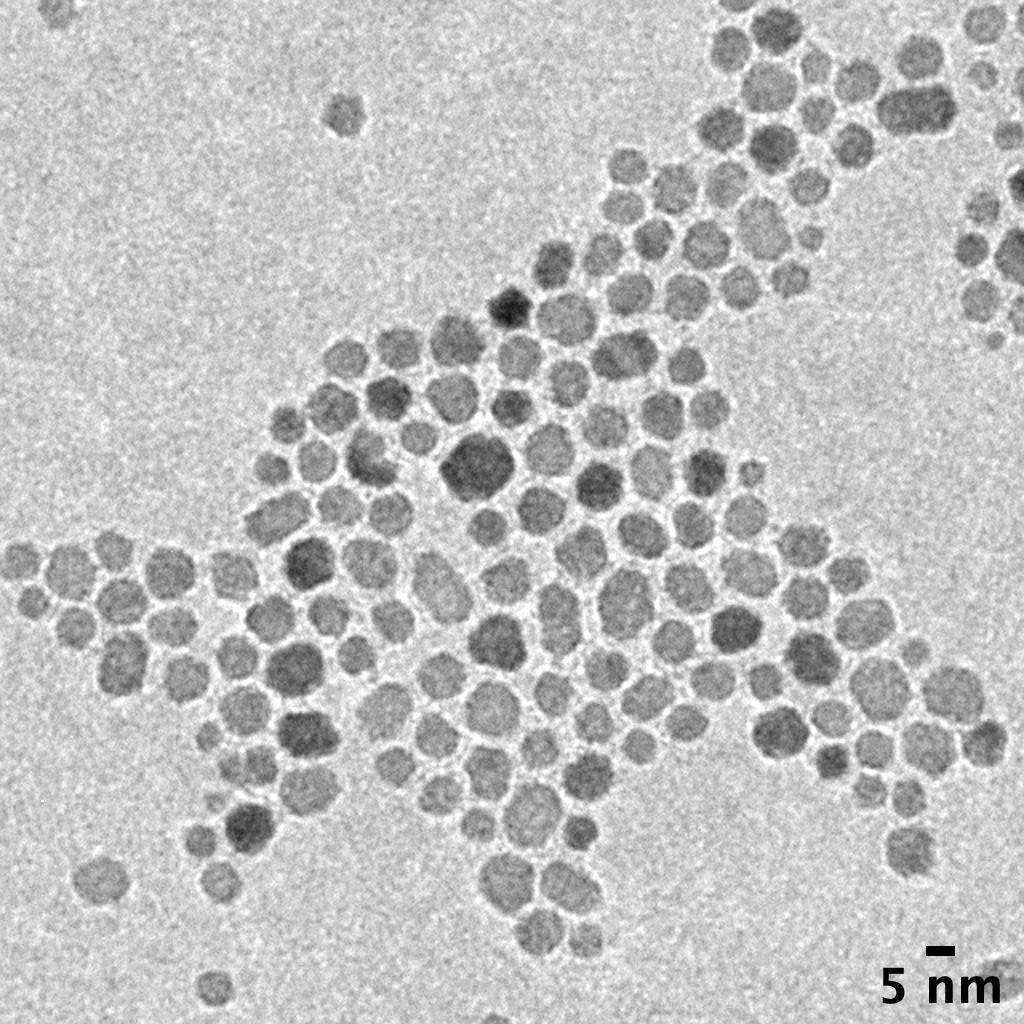
\includegraphics[width=\linewidth]{images/temh5.png}
	\end{subfigure}
	\begin{subfigure}[b]{0.25\textwidth}
		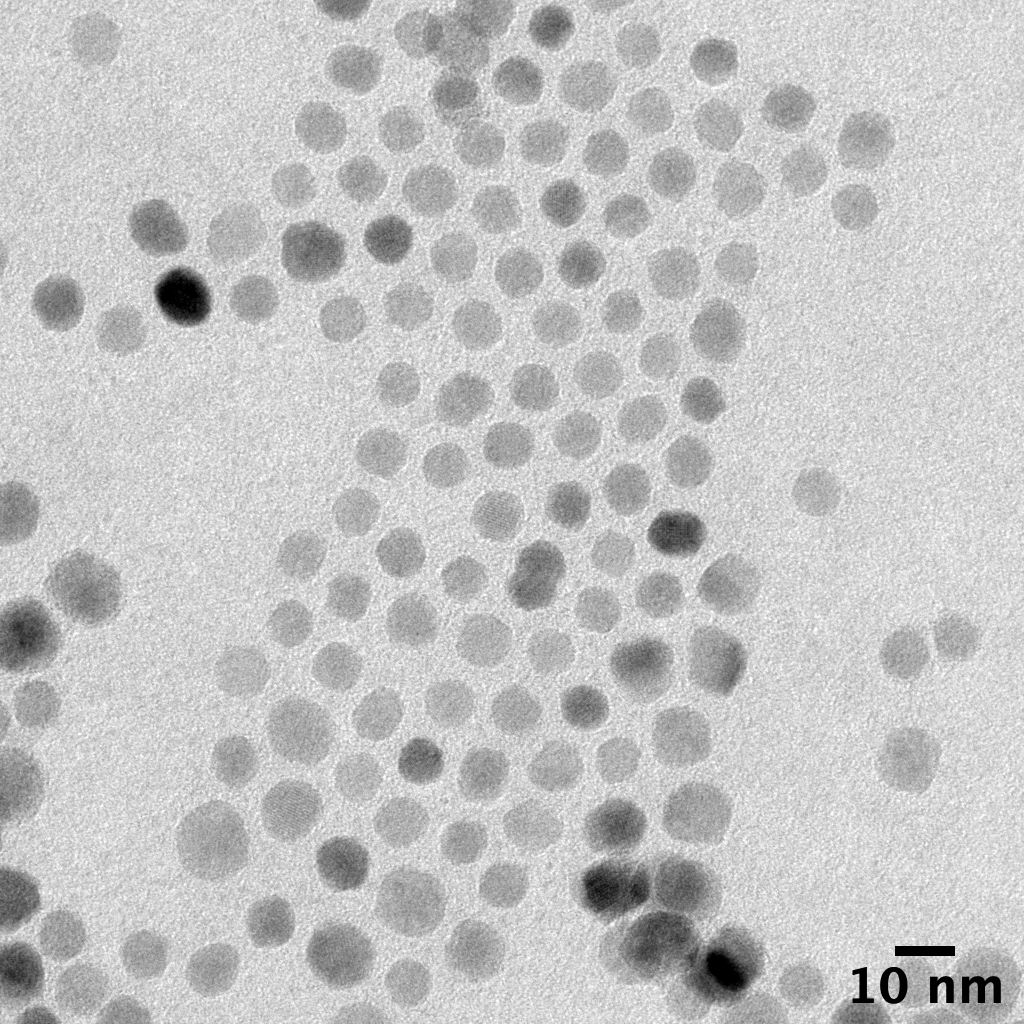
\includegraphics[width=\linewidth]{images/temh10.png}
	\end{subfigure}
	\begin{subfigure}[b]{0.25\textwidth}
		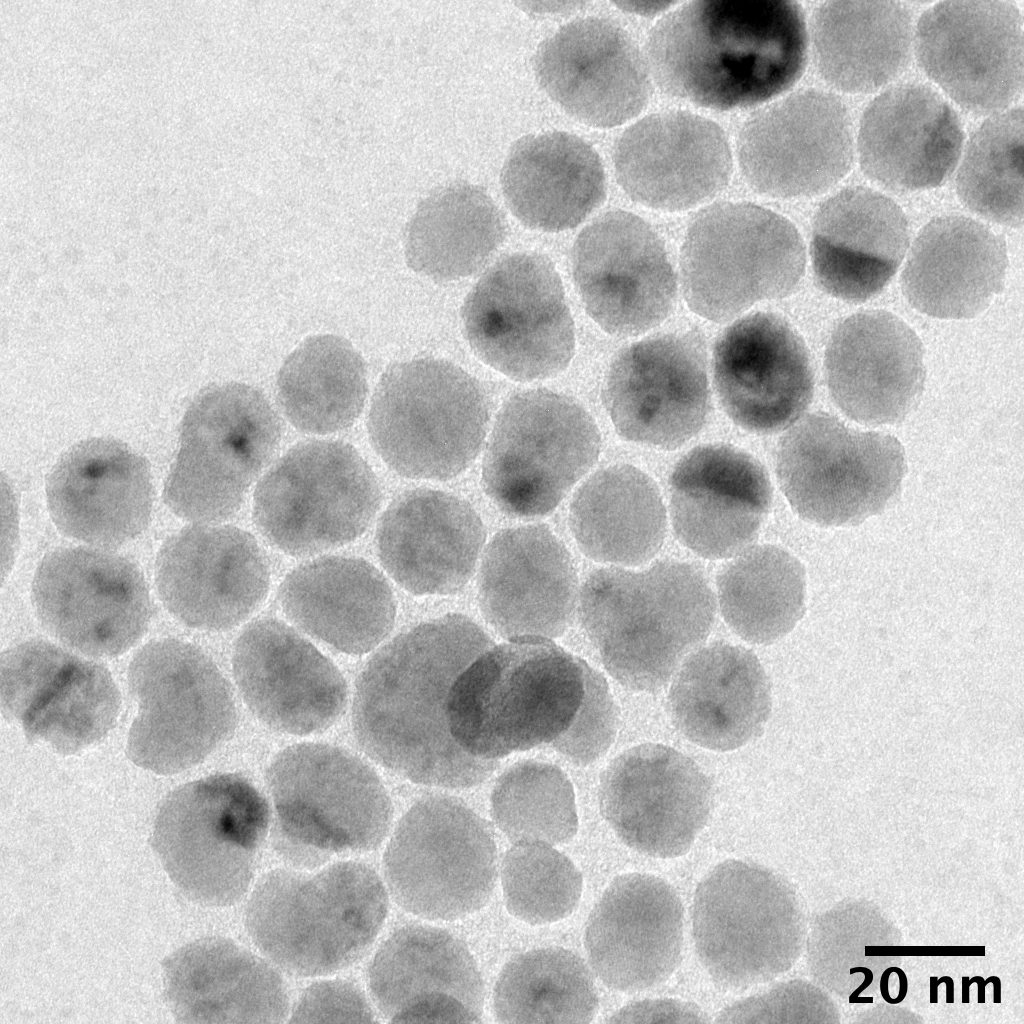
\includegraphics[width=\linewidth]{images/temh20.png}
	\end{subfigure}
\caption[TEM images of iron oxide nanoparticle]{TEM images of the iron oxide nanoparticles. From left to right: 5\,nm 10\,nm and 20\,nm nominal size in two different magnifications each (rows).}
\label{fig:tem}
\end{figure}

SAXS (small angle X-ray scattering) measurements of the prepared nanoparticle polymer foils were performed at the SSRL beamline 1-5. Samples were measured at 12\,keV  at two different spots for 5\,min each and averaged. A subtraction of the separately meassured polymer matrix background was performed and a size distribution of spherical particles with hard-sphere interaction fitted to the radial profile. The low-q area in the measurement is dominated by aggregate formation, which cannot be precisely quantified due to stray light and limited measuring range and is modeled for by a Guinier-Porod function, see \fref{fig:saxsps}  and  \fref{fig:saxspmma} \cite{percus1958,feigin1987,Ilavsky2009}.
The measurements do not show a clear and significant difference between the two polymer matrices. According to the regressions, the aggregates seem to have a radius of gyration of 20-30\,nm (the straylight limits the measurement validity in those small q areas) in both matrices, the Porod parameter $P$ of 2.5-3.8 suggests a dimensionality of the aggregates between 2 and 3 \cite{feigin1987,lili2005}. The radii of the form factor agree within the corresponding margin of error with the values determined by TEM measurements. The difference between the radius parameters of the structure factors and the form factor is most likely caused by the thin layer of oleic acid ligands between aggregating particles.


\begin{figure}[tp]
	\centering
	\begin{subfigure}[b]{0.3\textwidth}
		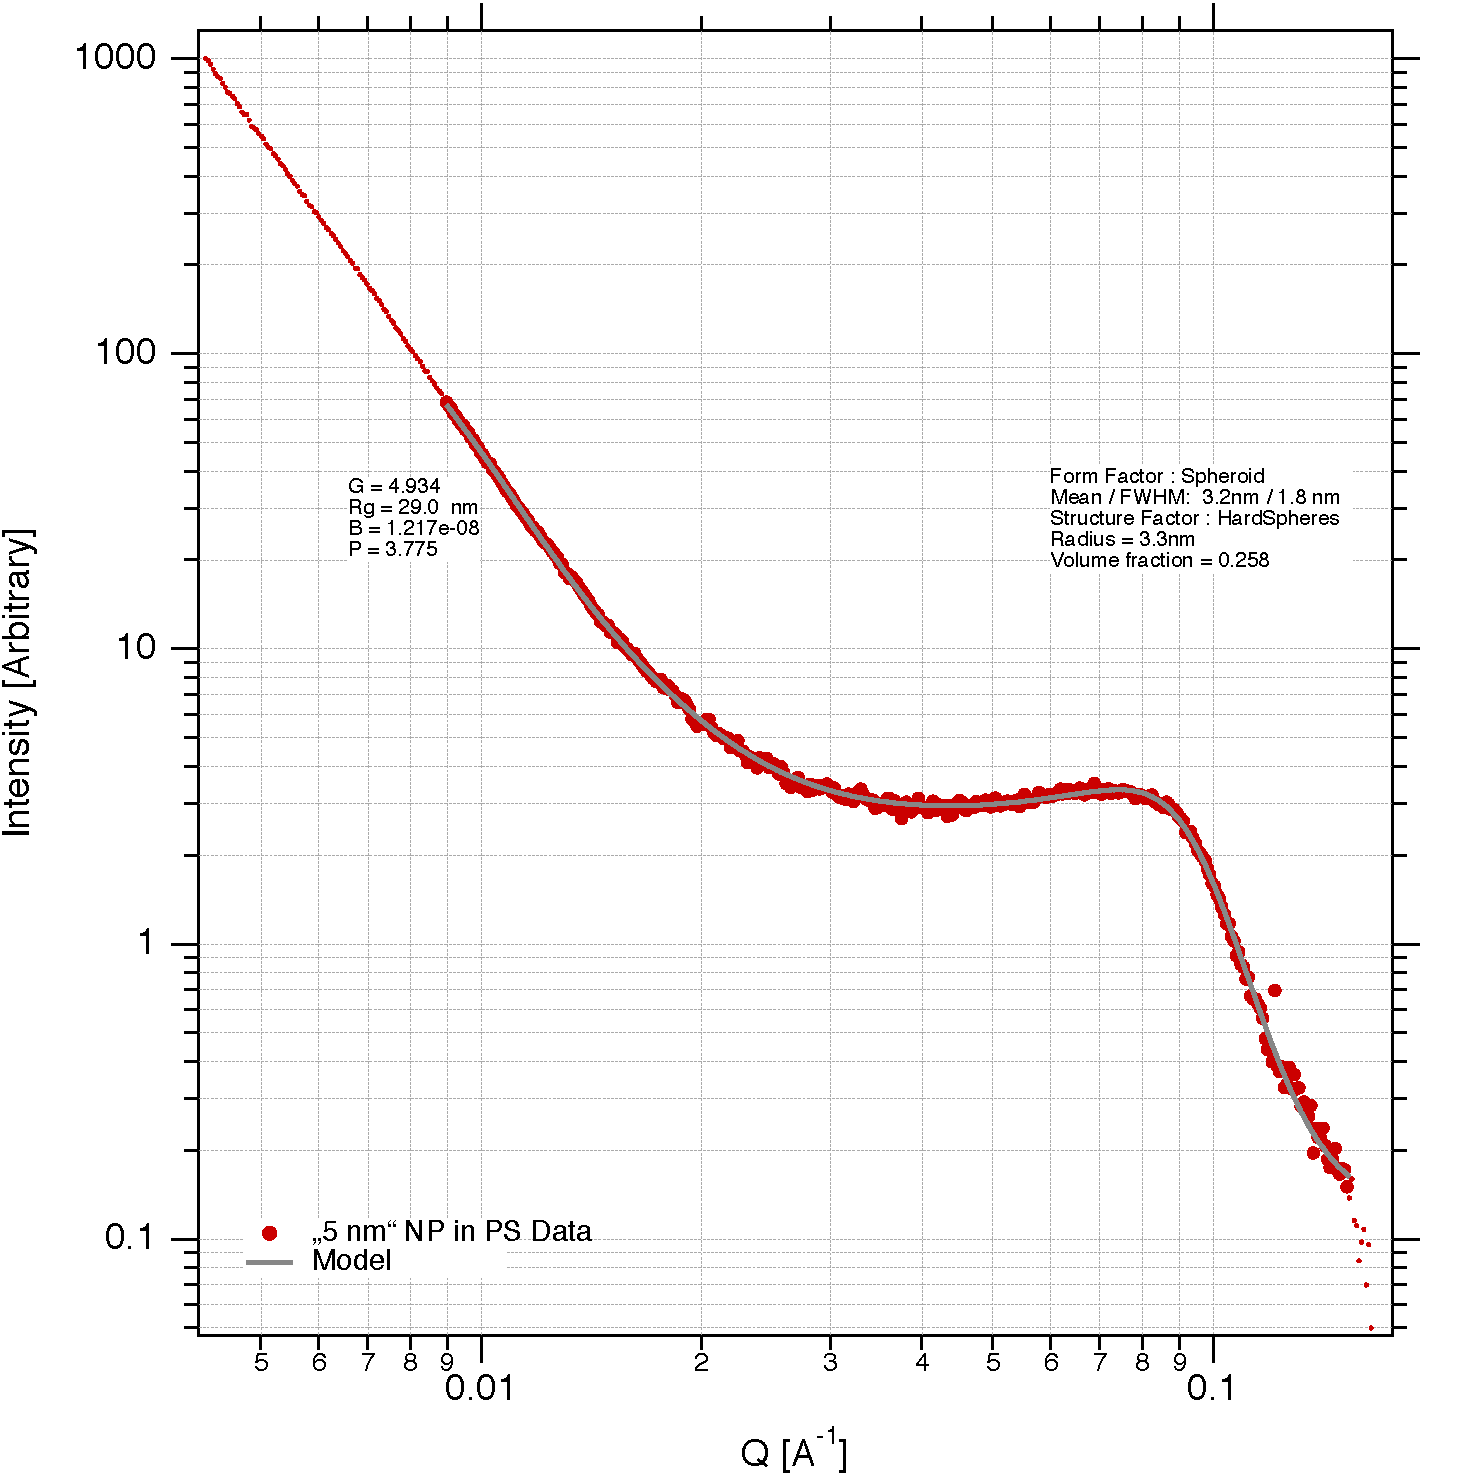
\includegraphics[width=\linewidth]{images/ps5.pdf}
	\end{subfigure}
	\begin{subfigure}[b]{0.3\textwidth}
		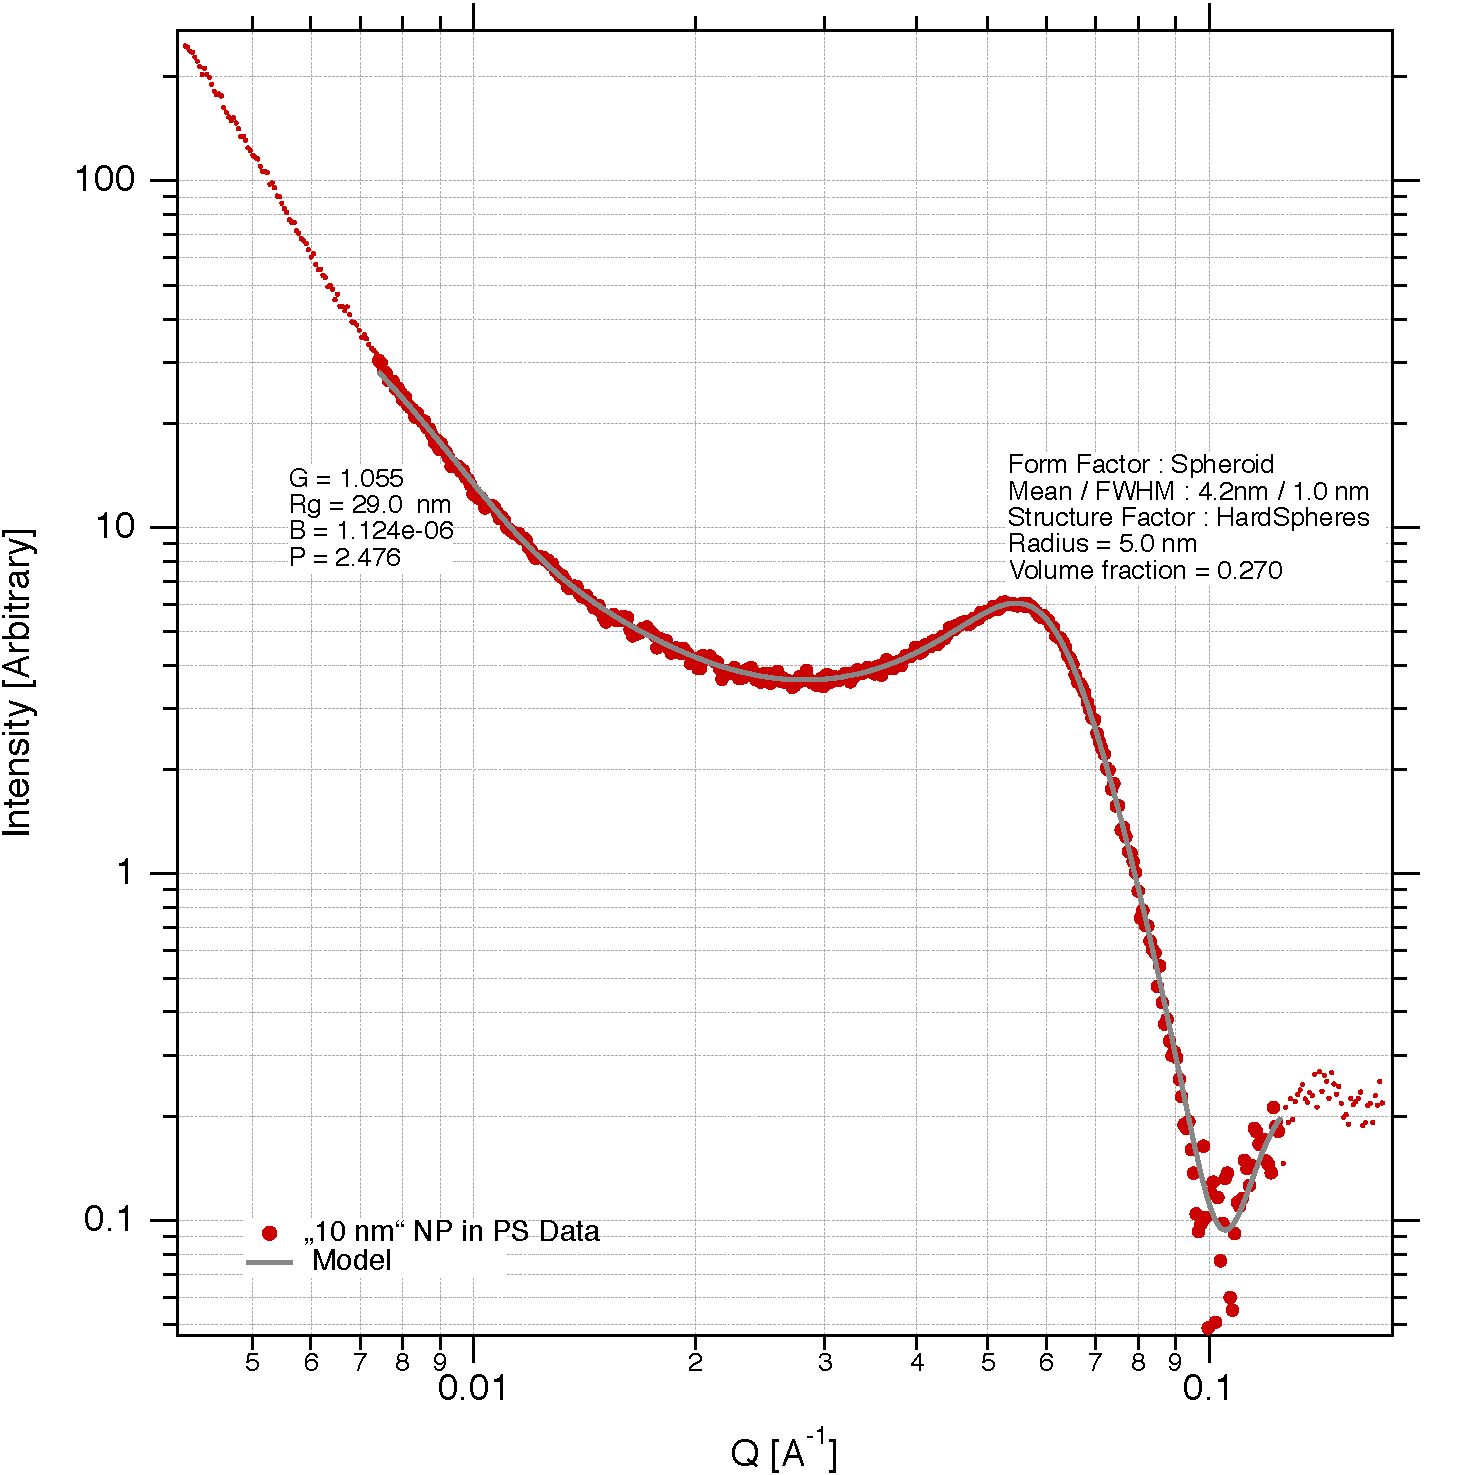
\includegraphics[width=\linewidth]{images/ps10.pdf}
	\end{subfigure}
	\begin{subfigure}[b]{0.3\textwidth}
		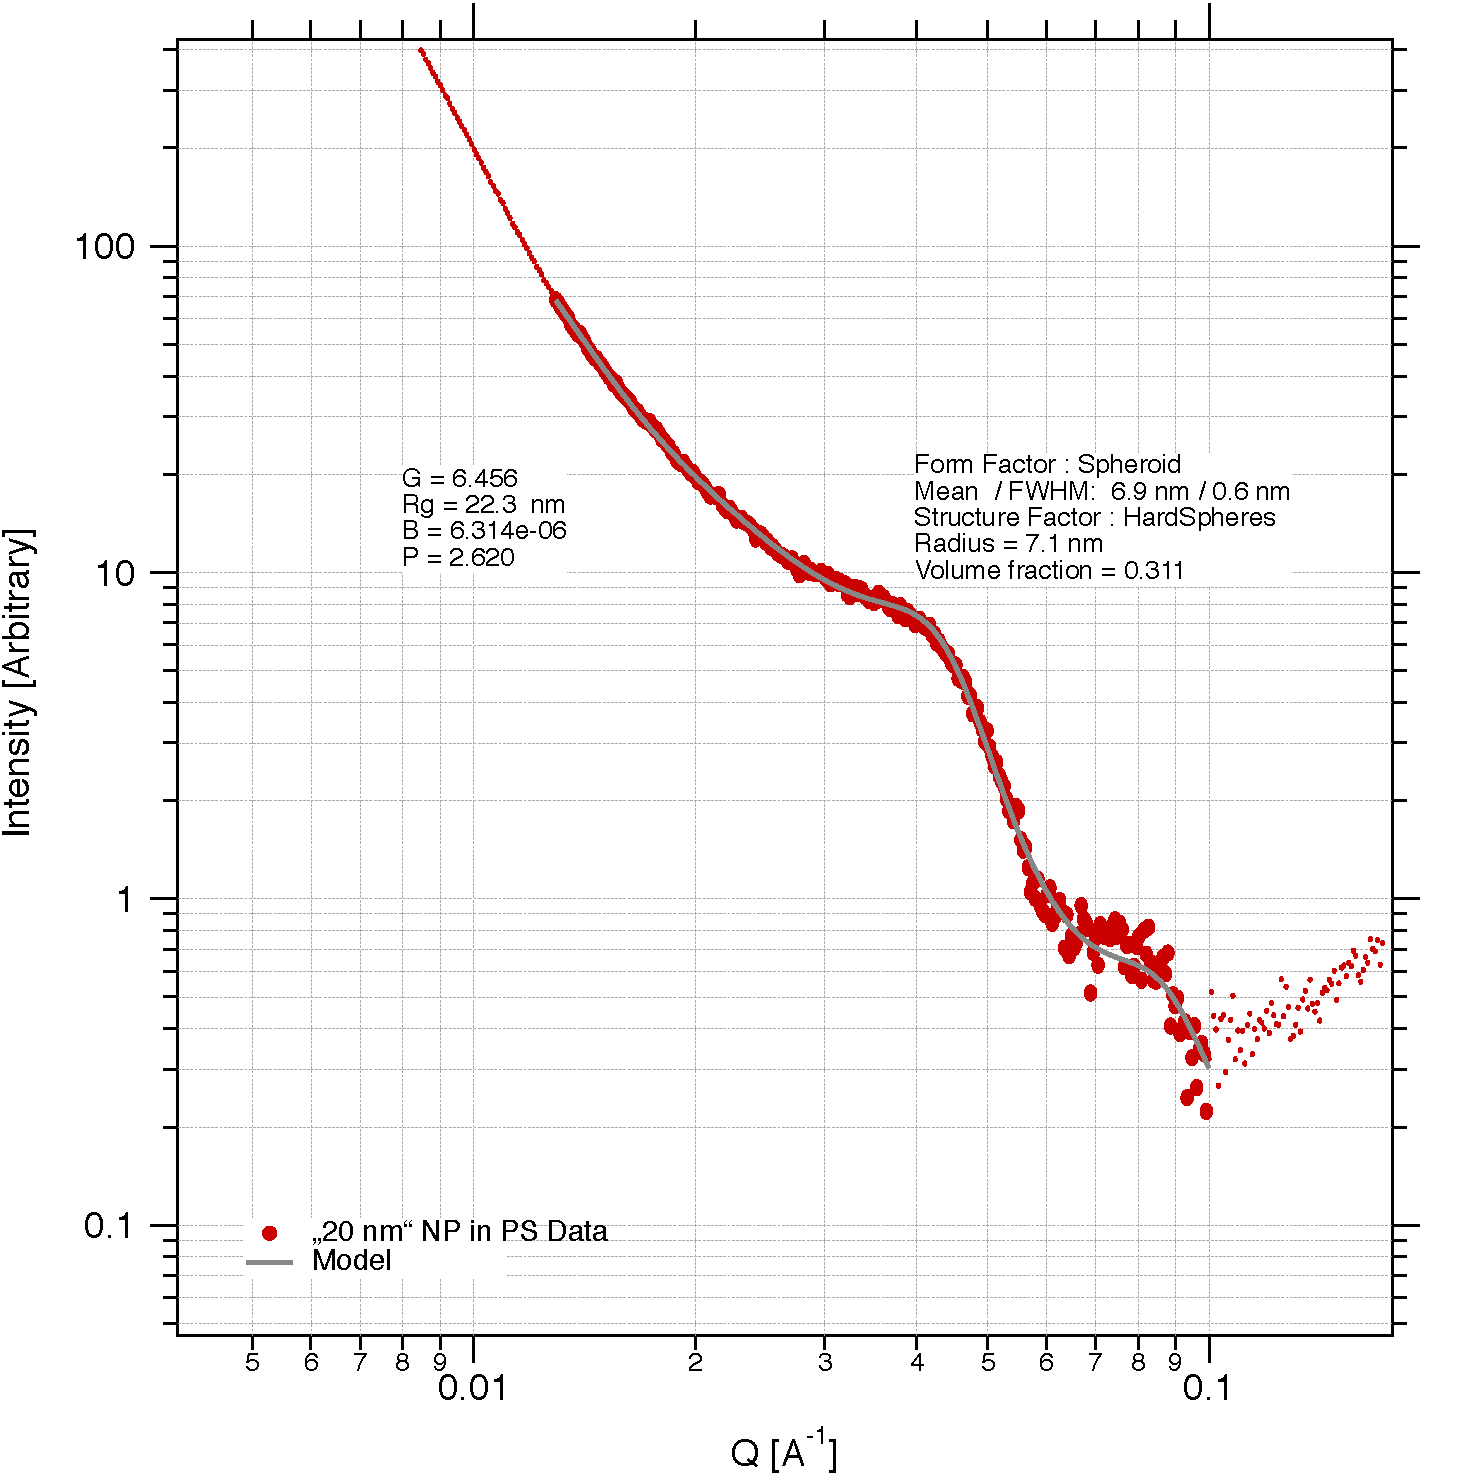
\includegraphics[width=\linewidth]{images/ps20.pdf}
	\end{subfigure}

	\caption[SAXS profile of iron oxide nanoparticles in polystyrene matrix]{SAXS profiles of nominal 5\,nm, 10\,nm and 20\,nm iron oxide nanoparticles in polystyrene matrix (left to right).}
	\label{fig:saxsps}
\end{figure}
\begin{figure}[tp]
	\centering
	\begin{subfigure}[b]{0.3\textwidth}
		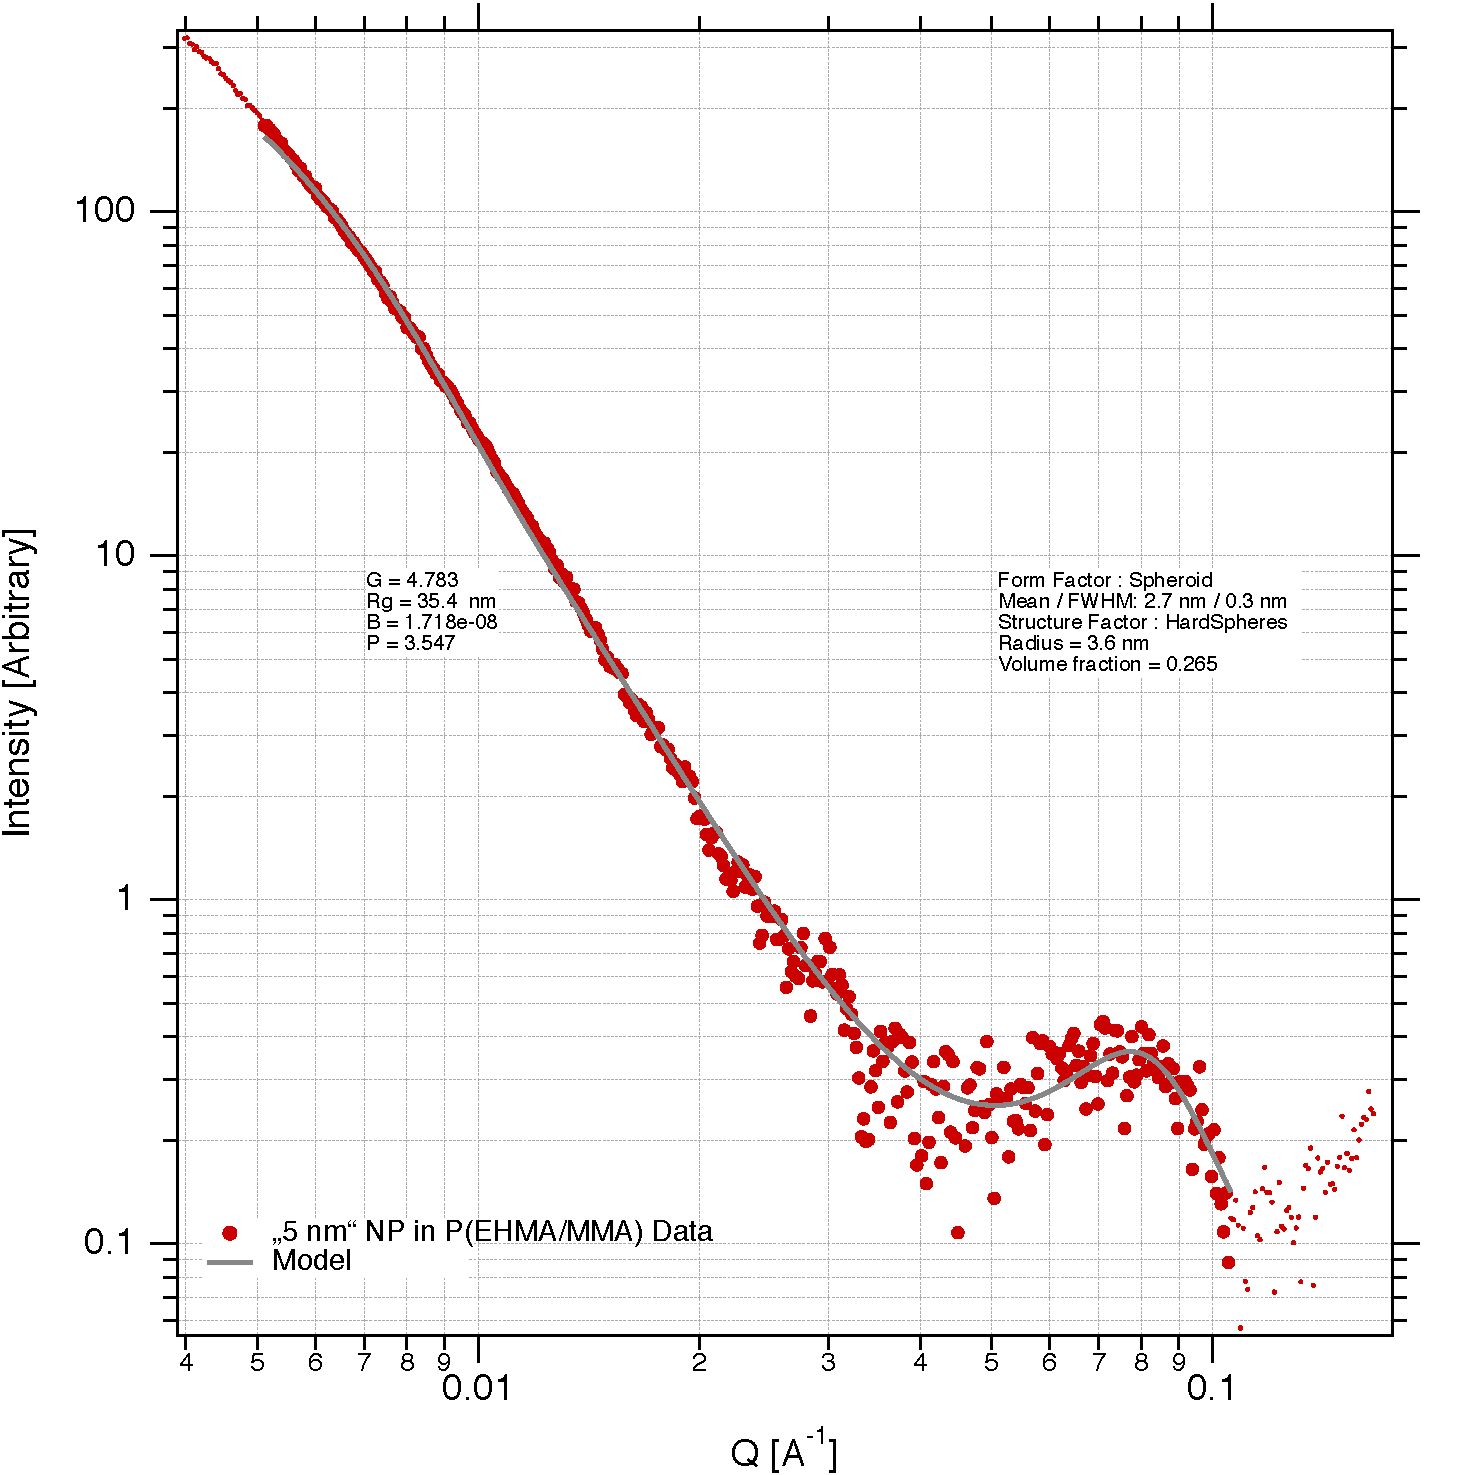
\includegraphics[width=\linewidth]{images/pmma5.pdf}
	\end{subfigure}
	\begin{subfigure}[b]{0.3\textwidth}
		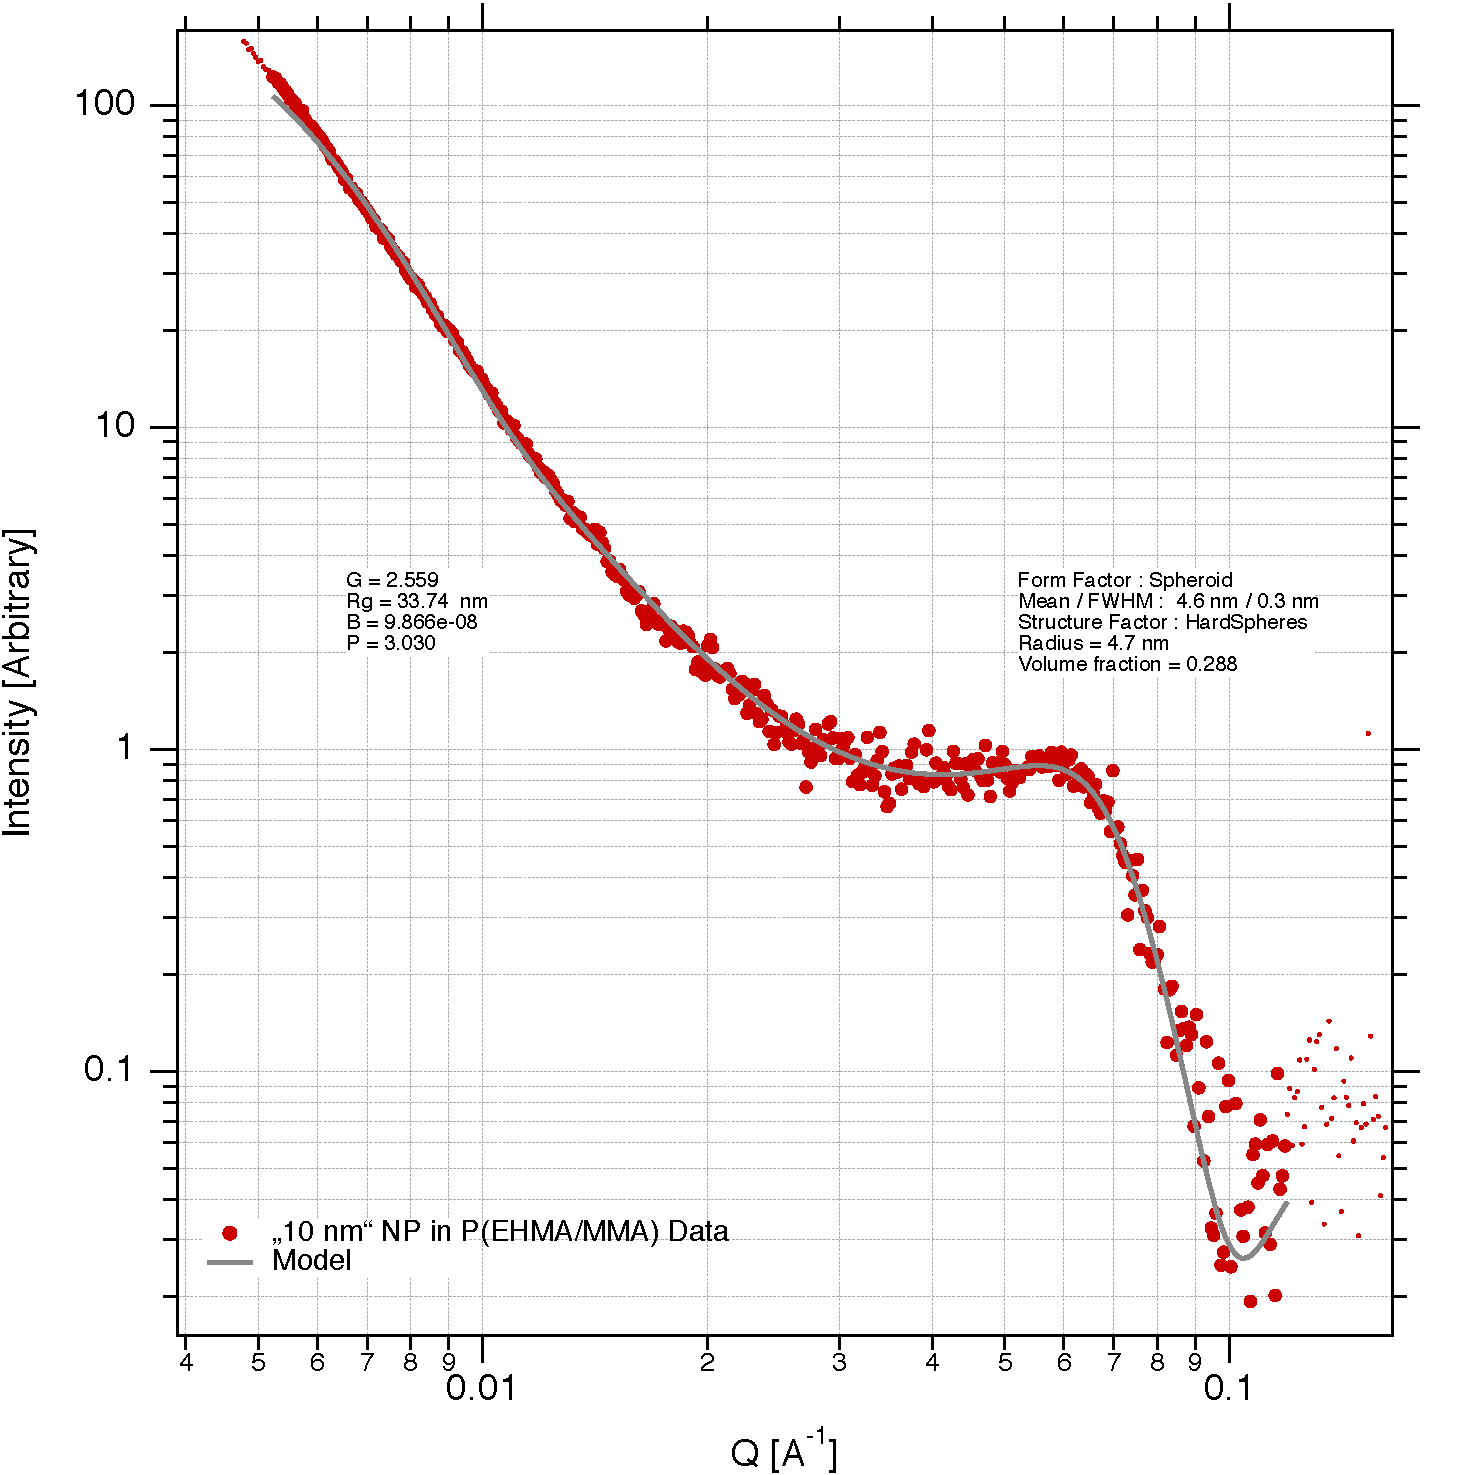
\includegraphics[width=\linewidth]{images/pmma10.pdf}
	\end{subfigure}
	\begin{subfigure}[b]{0.3\textwidth}
		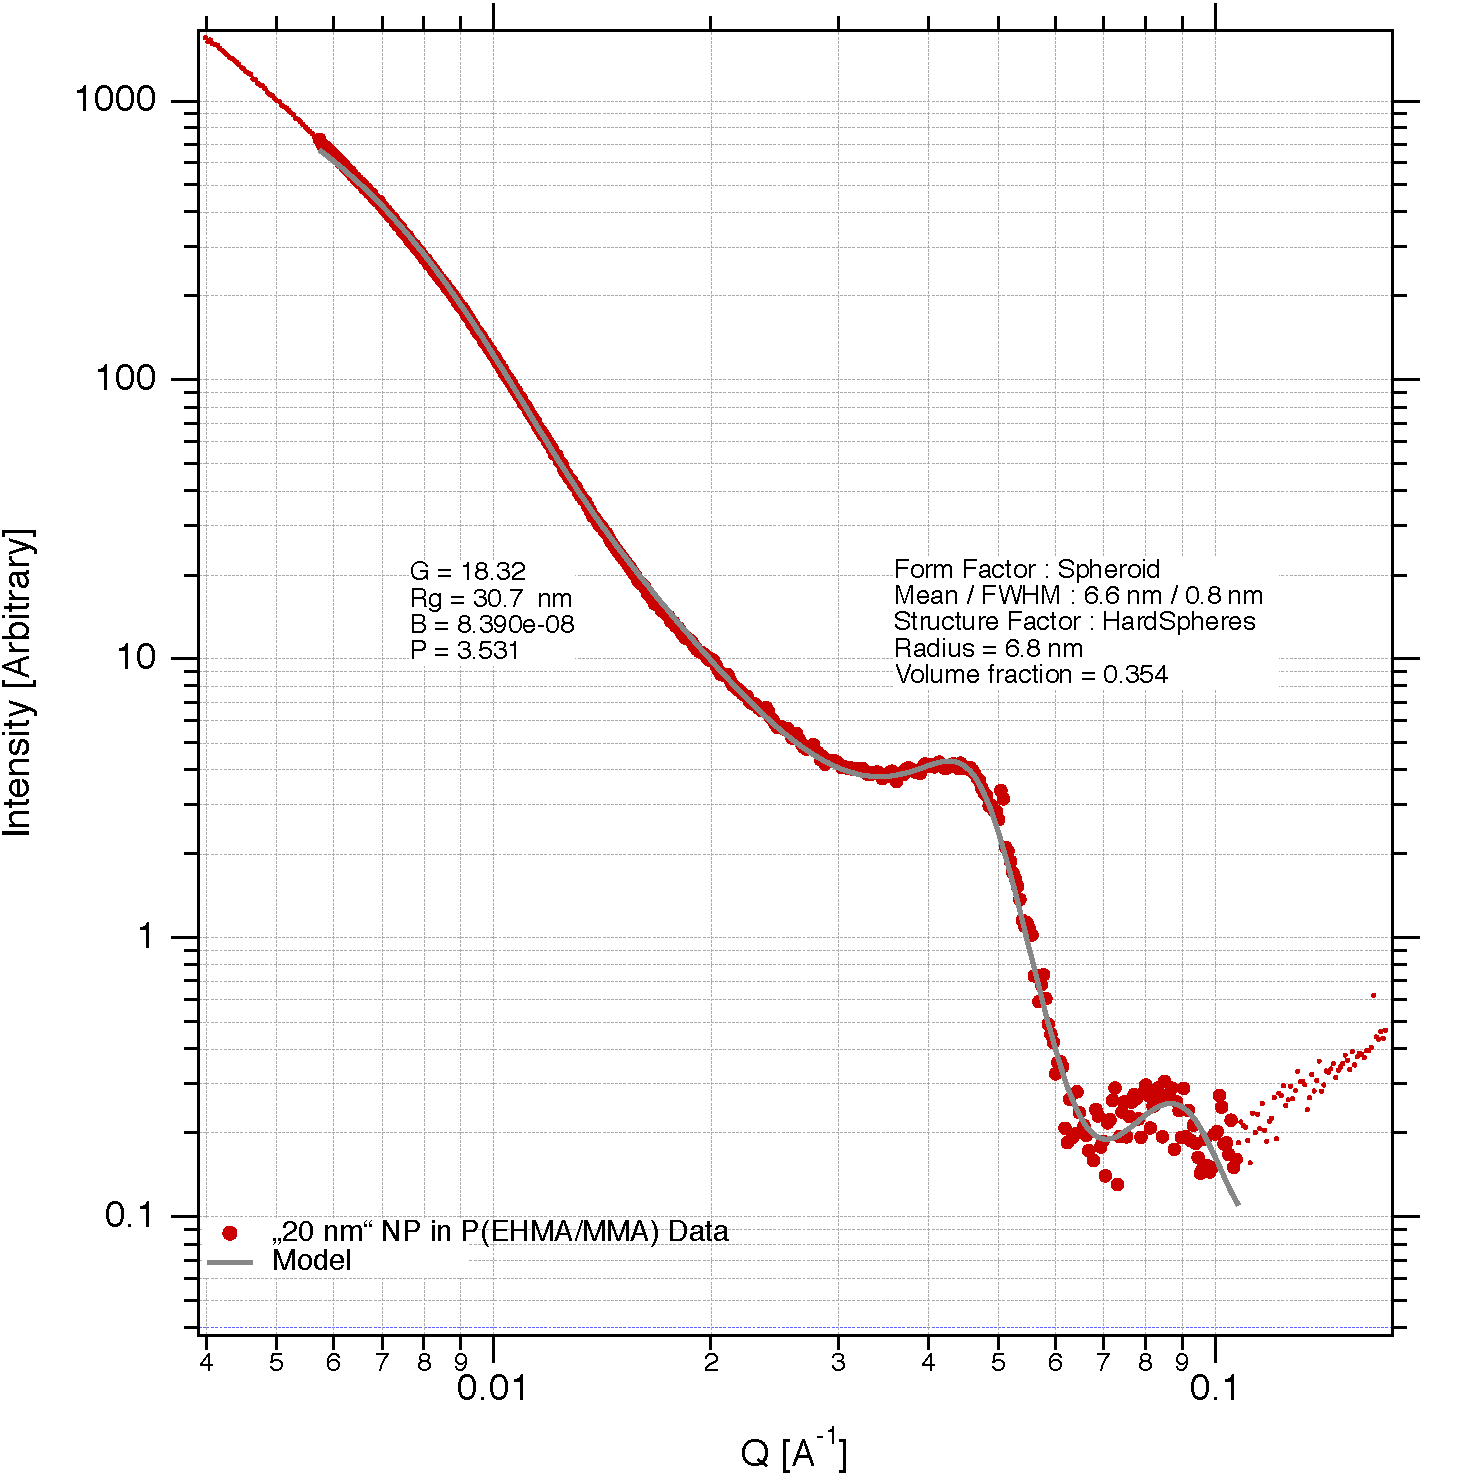
\includegraphics[width=\linewidth]{images/pmma20.pdf}
	\end{subfigure}
	
	\caption[SAXS profile of iron oxide nanoparticles in  Poly-(EHMA/MMA) matrix]{SAXS profiles of nominal 5\,nm, 10\,nm and 20\,nm iron oxide nanoparticles in Poly-(EHMA/MMA) matrix (left to right).}
	\label{fig:saxspmma}
\end{figure}
\subsection{Galliumarsenide Crystal Films}
The samples were prepared by Ben Reeves at the Stanford Nanofabrication Facility.
Using MOCVD, 50\,nm GaAs, 400\,nm AlGaAs as an etch stop and finally a 5\,\textmu m GaAs film were grown on an epi-ready (100)±0.1° GaAs substrate. The specimen was cut into 12\,mm\,x\,15\,mm pieces, each glued to an approx. 100\,\textmu m thick fused silica cover slip with the 5\,\textmu m film layer facing towards the silica. The substrate and the AlGaAs layer were selectively etched away via C6H8O7:H2O2 and HF:H2O wet etches, respectively. This left 5\,\textmu m thin GaAs films glued onto the the silica slides (see \fref{fig:gaas_sample}). 
A X-ray diffraction $\omega$-scan with copper K$\alpha$ (PANAlytical X’Pert Pro) shows the FWHM width of the (004) GaAs Bragg peak after mounting on the silica slides as 0.004°, indicative of high quality single crystals. 



\begin{figure}[tp]
	\centering
	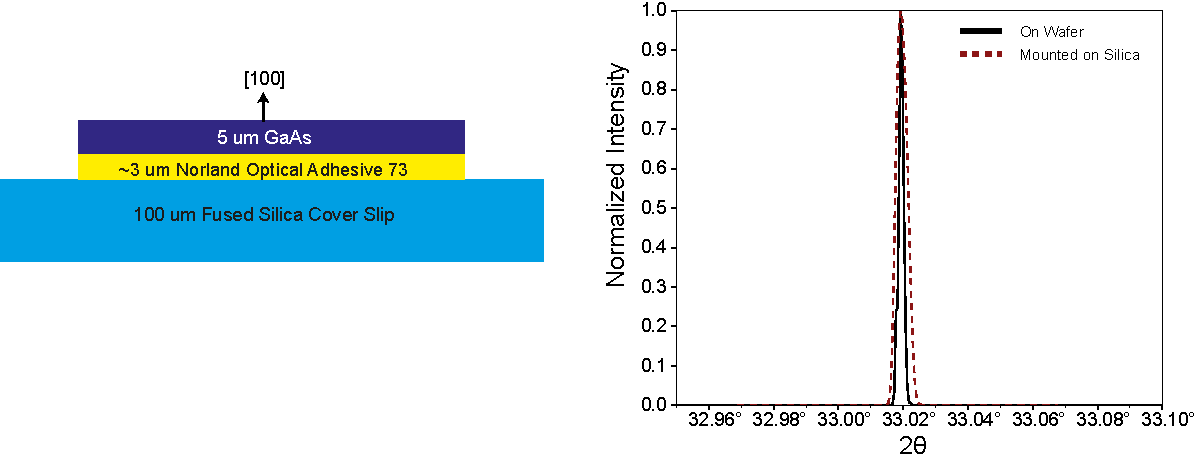
\includegraphics[width=0.8\linewidth]{images/gaas_sample.pdf}
	\caption[GaAs sample]{Sketch of the GaAs single crystal glued to a fused silica cover slip and Cu-K$\alpha$ XRD measurement of the GaAs (004) reflex, performed by B. Reeves, showing a single crystal. After mounting on the cover slip, the peak is slightly broadened, most likely by an slightly uneven thickness of the glue layer  leading to bending of the thin crystal.}
	\label{fig:gaas_sample}
\end{figure}

\FloatBarrier
\section{Setup of the Experiment}
The setup used at the experimental station EH5 at SACLA is shown in \fref{fig:setup}. 

The FEL provided approximately 10\,fs long hard X-ray pulse with $\approx 10^{11}$ photons at 11\,keV (just above the gallium K-edge and below the arsenic K-edge, see \fref{tab:elements}) and 30\,Hz repetition rate \cite{tono2013}. The beam was focused by the \textit{100\,exa} KB nano-focusing system. The focus spot along the beam direction was found by optimizing the strength of (non-linear) amplified spontanous emission (ASE) of a copper foil, resulting in focal FWHM of 200\,nm vertical/100\,nm horizontal (as determined by a wirescan) \cite{yumoto2020,handa2010,yoneda2015}.

The sample was mounted in a 45° angle to the beam on a stack of two rotational/two translational/two rotational/three translational stages to allow scanning of the sample, to ensure perpendicularity of the scanning directions to the beam to stay within the Rayleigh length (approx. 100\,\textmu m horizontal/200\,\textmu m vertical) while also ensuring a parallel alignment of the sample surface to one of the detectors. 

Overall, two MPCCD detectors were used: A dual detector with two tiles, each 512x1024 pixels perpendicular to the FEL beam in a distance of 1\,m and a \textit{Short Working Distance} octal detector, consisting of eight 512x1024 pixel tiles, parallel to the sample surface in a distance $d_{octal}=$14-50\,cm. To suppress absorption and more importantly, air scattering, a vacuum pipe with Kapton windows was installed in between the sample and the dual detector.
An L-shaped aluminum plate was installed to reduce stray light as well as to allow mounting of the beamstop and filters between sample and detectors.

The samples were scanned with a mean step size of 20\,\textmu m in horizontal direction (fast scanning direction) and 20\,\textmu m in vertical direction between shots. The step size was chosen based on the crater size visible with an optical microscope of approximately 5-10\,\textmu m for the samples and energies used in the experiment.

\begin{figure}
	\centering
	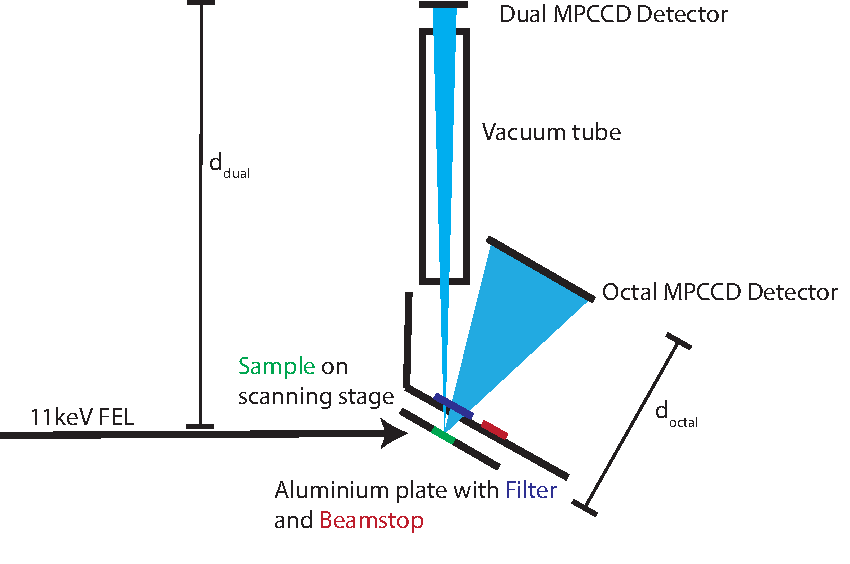
\includegraphics[width=0.75\linewidth]{images/setup.pdf}
	\caption[Experimental setup at SACLA]{Experimental setup at SACLA: The sample is mounted on a scanning stage and aligned to stay in focus during the scan and be parallel to the octal MPCCD detector, which is in a distance $d_{octal}$. The angle between incoming FEL and Sample is 45°. Behind the sample, a stray light filter, beamstop and (depending on the sample) a filter foil is installed. The dual detector is mounted $d_{dual}$=1\,m away from the sample perpendicular the the FEL beam. To reduce air scattering, a vacuum tube is installed in the path from sample to dual.}
	\label{fig:setup}
\end{figure}
\paragraph{Imaging the Focus}
To image the focus, one of the following foils with purity >99.99\% was mounted on the sample holder: 500\,nm iron (Goodfellow), 10\,\textmu m iron (Nilaco), 5\,\textmu m (Nilaco) and 20\,\textmu m (Goodfellow). The fluorescence was recorded using the dual detector at a distance of $d_\text{dual}$=1\,m.
The X-ray beam was attenuated by 0.4\,mm silicon, resulting in 20-30\,\textmu J  energy at the sample for pulse energies at the upstream energy monitors of 400\,\textmu J \cite{yabashi2015,tono2013}.
\paragraph{Imaging Nanoparticles}
For imaging the prepared iron nanoparticle and reference samples, the octal detector, which was the main imaging detector for these samples was moved to $d_\text{octal}\approx$43\,cm. The vacuum tube in front of the dual detector was partially removed to avoid mechanical interference. The sample was slightly moved out of focus along the beam direction by 400\,\textmu m instead of using any attenuation to increase the number of fluorescence photons. In between the nanoparticle samples, a single 10\,\textmu m iron foil measurement using the dual detector was taken to confirm the beam conditions.

\paragraph{Imaging Crystals}
For imaging GaAs single crystal samples, the distance between the octal detector and the sample was shortened to $d_\text{octal}\approx$14\,cm (with the vacuum tube between the dual detector and the sample removed). A 25\,\textmu m zinc filter was installed on the filter holder to reduce the amount of non-fluorescence photons (air scattering, coherent scattering in the sample etc.), as well as gallium K$_\beta$ fluorescence on the detector. The crystal surface was aligned to be parallel to the detector plane, and the scanning directions were aligned to be parallel to the crystal surface within less than 1°. The X-ray beam was attenuated by 0.4\,mm silicon.

\section{Data Processing and Analysis}
As the amount of recorded data is huge, an efficient strategy for filtering on shots, preprocessing the data to eliminate interference and finally reconstruction had to be implemented.
\subsection{Preprocessing}

\paragraph{Preliminary shot filtering}
A first rough filtering pass on the recorded data was done on the following criteria: Reported beam energy > 250\,\textmu J, beam energy in the hutch being not more than one standard deviation below the mean energy and the distance on the sample to the closest neighboring shot not being less than one standard deviation of the mean distance to the next neighbor for the sample (to remove shots with stopped, turning or still accelerating scanning motors). Furthermore, the scanning range occupied by the sample was identified by the fluorescence intensity on the octal detector and shots, where the X-ray beam does not hit the sample were removed. The remaining images were used to create spectra and perform photon counting.


\paragraph{Filtering for Impurities}
On some of the samples, areas can be identified where the relative fluorescence intensities at different energies change in the recorded data. An example is shown in \fref{fig:xrf}: For a 500\,nm thick iron foil, a spot can be seen where the intensity at 8\,keV is much higher than expected. As this is most likely due to impurities on the sample, those areas were identified and excluded from further analysis.

\begin{figure}
	\centering
	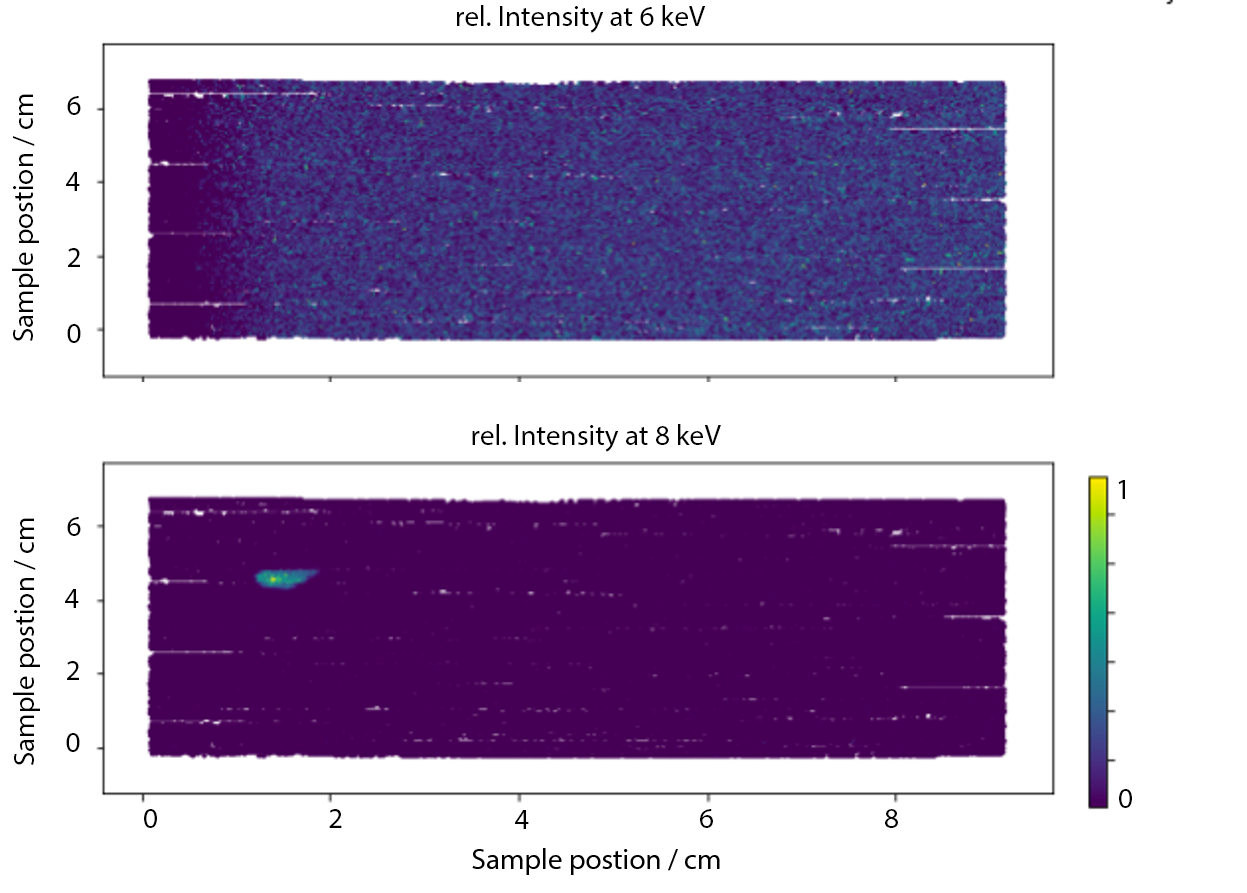
\includegraphics[width=0.7\linewidth]{images/xrf.png}
	\caption[Exemplary relative intensity of the 6 keV and 8 keV photon peak on the detector for different scanning positions on the sample]{Exemplary relative intensity of the 6 keV and 8 keV photon peak on the detector for different scanning positions on the sample. In this iron sample, a localized impurity, most likely copper, is clearly visible and can be masked out.}
	\label{fig:xrf}
\end{figure}

\paragraph{Detector masking}
Masks for both detectors were created based on the standard deviation over different dark images in a pixel not being more than than 4 standard deviations higher than the mean over all pixels (filtering out more noisy areas), the mean intensity over images recorded with a sample not being more than 3 standard deviations lower or higher than the mean as well as the extrema over the shots not being more than 3 standard deviations lower or higher than the mean. The masks were dilated by 5 pixels, examples are shown in \fref{fig:mask}.

\begin{figure}
	\centering
	\begin{subfigure}{0.2\textwidth}
		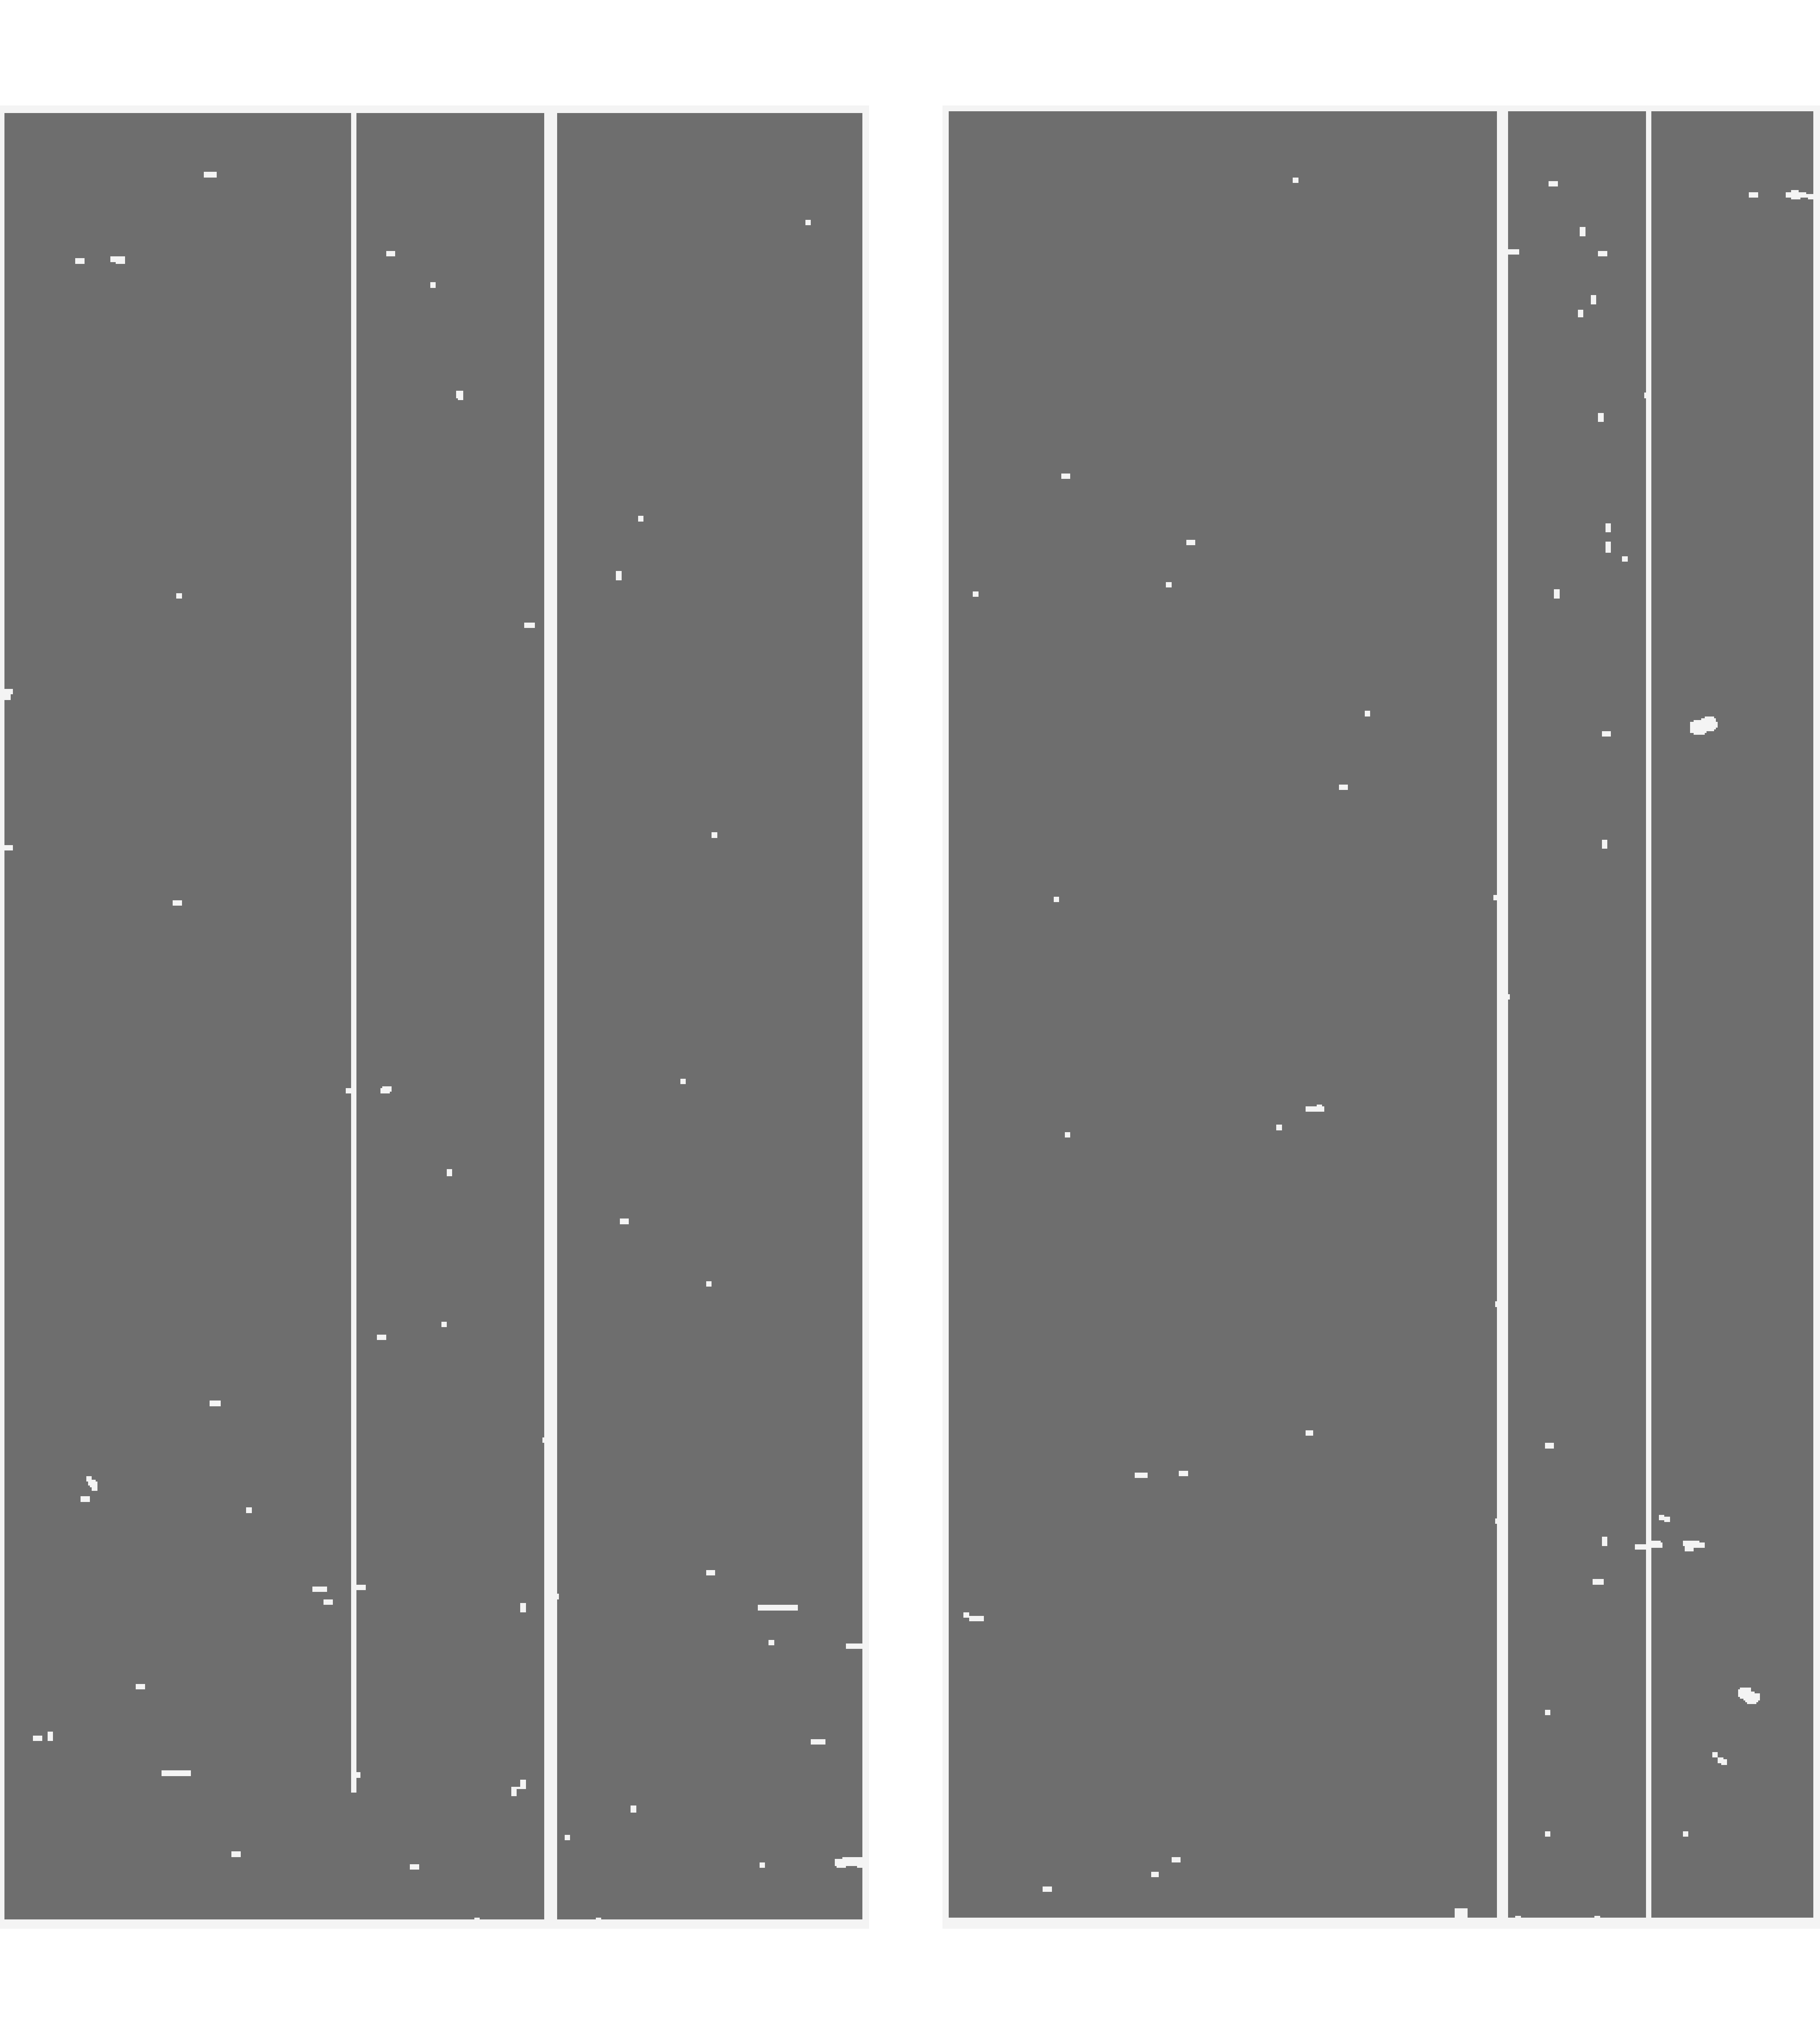
\includegraphics[width=\linewidth]{images/mask_dual.png}
	\end{subfigure}
	\hspace{1cm}
	\begin{subfigure}{0.2\textwidth}
		
\includegraphics[width=\linewidth]{images/mask_octal.png}
	\end{subfigure}
	\caption[Usable detector area]{Usable detector area (gray) of the dual detector for foil samples (left) and the octal detector (right) for NP samples after signal correction and statistical filtering. Masks are created by considering the intersection of good areas for each type of samples, in order be able to use the mask and therefore number of correlation pairs for samples that will be compared to each other.}	
	\label{fig:mask}
\end{figure}

\paragraph{Detector Artifacts}
During the experiment, an unnoticed failure of the electronics of the octal detector occurred, manifesting as periodic noise on most of the detector tiles at a much higher level than expected (see \fref{fig:octalissue} for an illustration). Not all columns of a tile or read-out port were affected, in contrast to common-mode effects more commonly encountered with CCD detectors. As the overall affected area of the detector is substantial and the noise leaks through the photon counting scheme by slightly influencing the probability of a pixel being considered a photon hit, causing correlations and therefore artifacts in the reconstruction in one direction, a correction was applied to the affected columns of affected tiles of the detector. For the correction, affected columns were first identified by filtering on the Fourier transform, neighboring effected columns are considered as a block and the medians over those blocks were calculated and subtracted. This scheme was chosen instead of the more commonly used portwise common mode correction due to the uneven strength of the artifact (see \fref{fig:app_correction} for a comparison). Using this correction reduced the artifact, but did not completely remove it. As the remaining artifact in the reconstructions is limited to low $q$ compared to the expected positions of the features of the samples and only two orthogonal lines, it can be masked out.


\begin{figure}[tp]
	\centering
	\begin{subfigure}[b]{0.45\textwidth}
		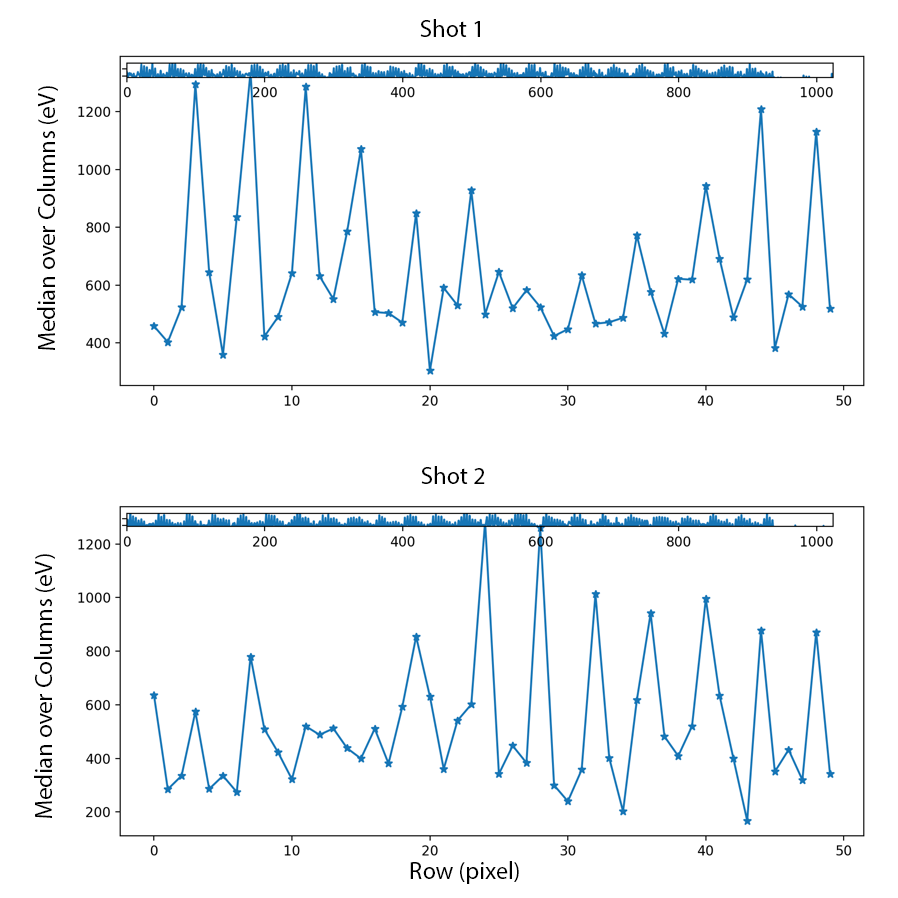
\includegraphics[width=\linewidth]{images/octalissue2.png}
	\end{subfigure}
	\begin{subfigure}[b]{0.45\textwidth}
		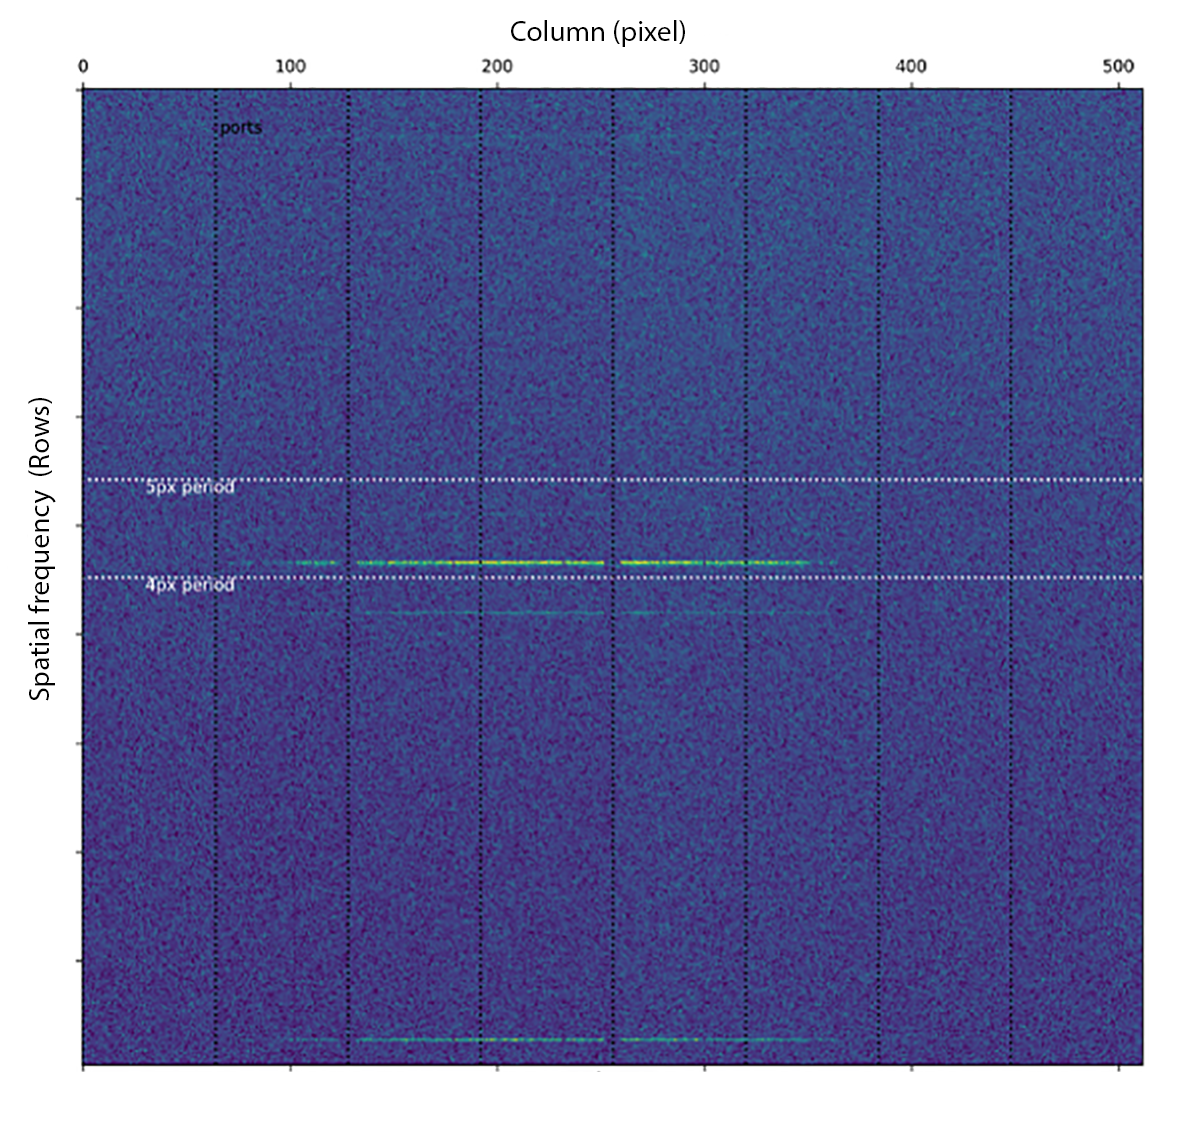
\includegraphics[width=\linewidth]{images/octalissue.png}
	\end{subfigure}
	
	\caption[Periodic noise on octal detector]{Periodic noise on octal detector after background subtraction: For two exemplary shots the median over columns of one detector tile is shown. A periodic noise is visible. The mean spatial spectrum (over the rows) for each column of the tile is shown on the right. The periodic noise is not uniformly affecting all the columns of the tile.}
	\label{fig:octalissue}
\end{figure}


\paragraph{Spectra}
The background subtracted and masked detector images were used to create spectra. The different samples were categorized into a smaller number of groups by the apparent similarity of the spectra/number of signal photons: The foil  data was grouped into three classes: one for copper foils, one for 10\,\textmu m thick iron foils and one for 500\,nm thick foils. The nanoparticle and single crystal data were assigned one class each.
On these spectra, a regression was performed.  The model consisted of peaks at multiples of the K$_\alpha$, K$_\beta$ and of the excitation energy with an initial FWHM of 500\,eV and intensities following a negative binomial distribution (signal) or Poisson distribution (scattering noise). To roughly approximate the charge sharing, a numerical convolution with a  window of the shape
\begin{equation}
	w (x)= (1-p)\delta(x)+\rect\left(\frac{x-1/2}{E_{signal}}\right)\frac{p}{E_{signal}}
\end{equation}
was included, thus smearing the peaks to lower energies with a strength parameter $p$ (initialized as 25\%). The mean squared difference the logarithmic values was minimized. With this regression, an estimate for the number of modes of the binomial distribution as well as for the mean number of signal and scattering photons was found.


\paragraph{Photon counting}
The mean number of signal and scattering photons found from the spectra as well as the peak width and the charge sharing point spread function for the detectors were used to find the thresholds for a classification of the pixel values into signal photon numbers for each of the groups as described in \fref{sec:chargesharing}. 
With the determined K$_\alpha$, K$_\beta$ and scattering intensities, 1000 images with 4096x4096 pixels were simulated with Gaussian charge sharing. The determined peak widths were used as the FWHM of the (assumed to be Gaussian) detector noise.  The number of signal photons corresponding with the highest probability to each energy was determined for bins of 10\,eV. 


\paragraph{Final shot filtering}
Before doing the reconstruction, a final filtering pass was performed on the images, keeping only those shots where the following criteria were fulfilled: 1)  the reported pulse energy was >450\,\textmu J, 2) the upstream measured mean photon energy within the pulse was within two standard deviations of the median over all pulses, 3) the ratio of the pulse energy in the experimental hutch to further upstream in the optical hutch was within one standard deviation of the mean, and 4) the ratio of the intensity on all 4 edges of the detectors as well as the total intensity on both detectors to the pulse energy to was not lower than two and not higher than four standard deviations of the mean.  For the last criterion, the total scanning area used was cut into equally sized squares with a side length of 1/100th the horizontal scanning range and the filtering was done for all shots within each of those squares. This increased the statistics over a shot-wise filtering and proved sufficient to remove remaining bad areas on the sample (such as cracks resulting from previous shots) as well as areas where shadowing of the detector due to the sample holder might have occurred.




%XXX
%As shown in \fref{fig:spectrum}, the background corrected and masked spectrum of the detector shows peaks at multiples of the %fluorescence and excitation energy with a FWHM of .... . 


%As discussed in \fref{chap:simulation}, the number of fluorescence photons can be estimated...


% Raw Data
% Spectrum
% Peaks


\paragraph{Crystal orientation}
For determining the relative orientation of the crystal with regards to the detector, Kossel lines as described in \fref{sec:kossel} can be used. This can either be done by reprojecting the planar detector onto a sphere by an inverse gnomonic projection and determining circle center and radius, eg. by an Hugh-Transform, or by a fitting conic sections to the lines on the planar detector \cite{morris1968,morawiec2016,faigel2016,herron2018}. As the observable curvature of the Kossel lines on the detector in an IDI setup is small and therefore the circles are difficult to determine, the second method was chosen. A semi-automatic alignment program was developed (\fref{fig:kosselfit}) to aid with the procedure.

For each sample, the images were split into sets of 5000 shots. After filtering for hot pixels and cutting bellow a noise threshold of 2\,keV, the mean was taken. To better distinguish the Kossel lines from the uniform fluorescence, a Gaussian blurred version ($\sigma$=20\, px) was subtracted (see \fref{fig:kosselgaasmean} for examples). The Kossel lines were roughly identified manually and the local maxima in the 20x20\,px surrounding block of an identified area were considered as points on the Kossel line. A least-square regression was performed,

\begin{equation}
	\arg\!\min_{R,t} \sum_{r} \min_{q\in Q} \left\Vert \frac{2 d  \left( \vec{r} - \vec{t} \right) \cdot \vec{Rq}}{\left|\vec{q}\right| \left| \left(\vec{r}-\vec{t}\right)\right|} -\lambda \right\Vert_2^2 \,,
\end{equation}
with
$\vec{q}$ a reciprocal lattice vector and element of the allowed reflections $Q$, wavelength $\lambda$ and lattice constant $d$, to find
 the optimal angles of the rotation matrix $\vec{R}$ and the detector translations $\vec{t}$.
 


\begin{figure}
	\centering
	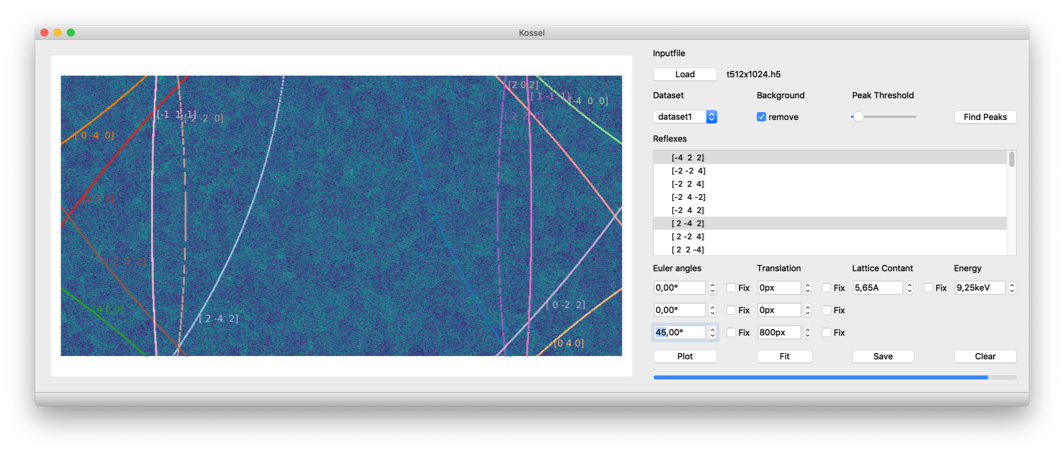
\includegraphics[width=0.8\linewidth]{images/kosselfit.png}
	\caption[User Interface for Kossel line based alignment]{User interface created for performing a regression of the detector orientation and position to the Kossel lines visible in experimental data. The lines can be automatically identified,  be  manually modified afterwards and the reflections considered selected. This tool is used to perform the alignment for the GaAs single crystal samples.}
	\label{fig:kosselfit}
\end{figure}





\subsection{Reconstruction}
For the foil data, the small angle approximation is valid and each pixel approximately covers the the same solid angle, permitting using a pixelwise correlation (after normalization by as described in \fref{sec:normal}) as a reconstruction of $|S(q)|^2$.
For the nanoparticle data, the maximum recorded angles are higher and at the limit of the small angle regime, resulting in $\delta q_x,_y$ between neighboring pixels being lower for pixels further of axis. Therefore, for each pixel the $q_x,q_y$ values were calculated and an explicit correlation according to \fref{eq:correlation} was performed.
For the crystal data, a full three dimensional correlation of the rotation and offset corrected data was performed using the resampled FFT-based approach.


\section{Results of the Experiment}
Applying the aforementioned preprocessing and analysis steps to the recorded fluorescence images for all three classes of samples leads to results as follows. 
\subsection{Imaging the Focus}

The regression of the spectra (\fref{fig:spectrafoil}) resulted in a mean K$_{\alpha}$ photon count per pixel of 0.004$\pm$0.001 (500\,nm iron foil) to 0.041$\pm$0.001 (20\,\textmu m copper foil). The mode number could not be reasonably estimated for the 500\,nm iron sample due to the influence of air scattering and fluorescence stemming from the experimental setup and low number of signal photons. For the other samples, the regression provided estimates in the range of 15-25 modes. The charge sharing approximation parameter $p$ was found to be 0.43$\pm$0.01, meaning about 40\% of the photon hits were affected. The simplifications of assuming a uniform charge cloud by using a convolution windows with a flat side lobe led to disagreement between the slightly curved histograms and the flat regressions in the valleys between integer multiples of the single-photon energy. This is no longer present in the spectra simulated with a Gaussian charge cloud (see \fref{fig:thresholdsfoil}) for an example.

The reconstructions were performed once without discretization and only applying a threshold of 1500\,eV and once with discretization into photons using the thresholds found in the simulation of the spectra. Without discretization, strong artifacts were visible in the reconstruction, which were mostly reduced by the applied photon counting (see \fref{fig:foil_photonmodes} for a comparison).

\begin{figure}
	\centering
	\begin{subfigure}[b]{0.45\textwidth}
		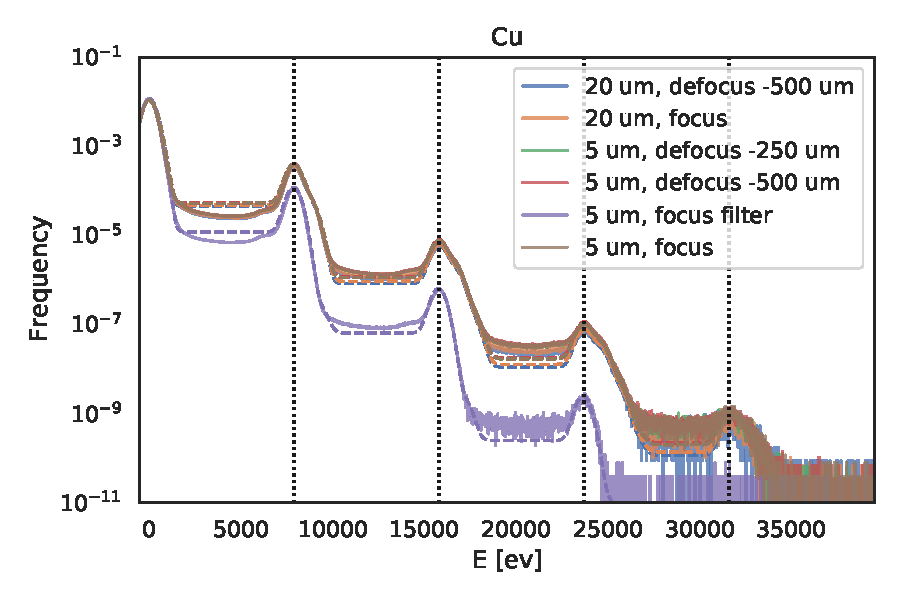
\includegraphics[width=\linewidth]{images/spectrum_foil_cu.pdf}
	\end{subfigure}
	\begin{subfigure}[b]{0.45\textwidth}
		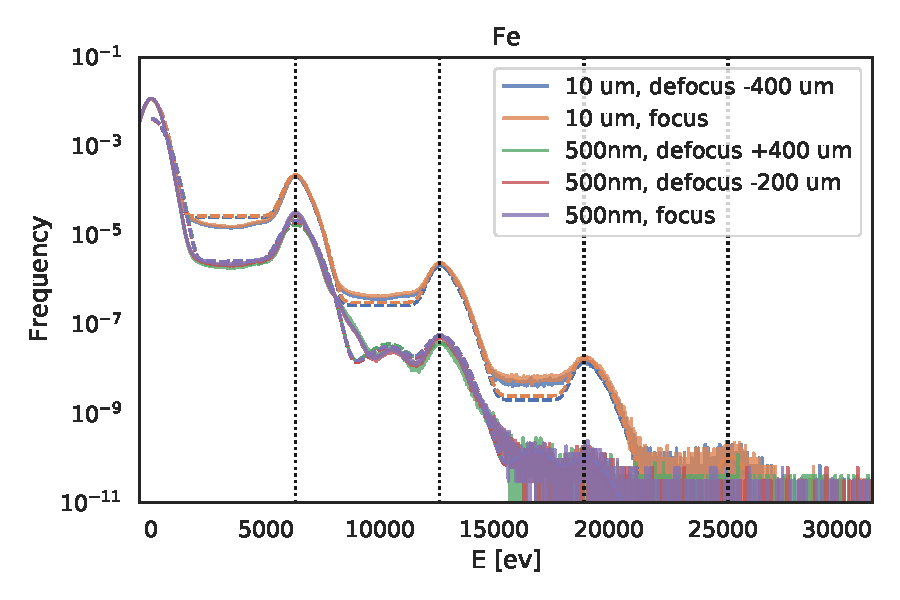
\includegraphics[width=\linewidth]{images/spectrum_foil_fe.pdf}
	\end{subfigure}
	\caption[Spectra of fluorescence using foil samples ]{Spectra of fluorescence using foil samples (left for copper, right for iron) and best fit of the regression using an approximated charge sharing.}
	\label{fig:spectrafoil}
\end{figure}


The excited volume can be approximated in horizontal direction as a rectangular function with a width of $\sqrt{2}$-times the thickness of the foil used, due to the 45° angle, as the horizontal FWHM of the focus is much smaller than the thickness of the foil and ignoring absorption.  In the vertical direction, the volume is limited by the FWHM of the focus and can be roughly approximated to be Gaussian. 
In a small-angle approximation, the reconstruction is the magnitude squared of the 2D Fourier transform of the volume. As the magnitude squared of the Fourier transform of a Gaussian with FWHM $f$ is another Gaussian with FWHM $\frac{4\sqrt{2}\log{2}}{f}$ and of a rectangular function\footnote{If the foil were thicker, the absorption length $a$ could not be ignored and the more complicated $\left|\mathscr{F}\left(e^{-\frac{x}{a}} \Pi \left(\frac{x}{w}\right)\right)\right|^2 \propto \frac{\cosh \left(\frac{w}{a}\right)-\cos (q w)}{a^2 q^2+1}$
	could be used instead.} with width $w$ is proportional to $\sinc^2{\left(\frac{q w}{2}\right)}$, a 2D least-squares regression of the product of those functions is performed on the reconstructed image to estimate the focal FWHM \cite{butz2015}. As the horizontal direction is under-sampled, the horizontal profile will not be resolved in the reconstruction.  The function used for the regression is sampled at 25x the resolution in both directions and averaged. This corresponds to a convolution with a rectangular sampling kernel and reduces the effect of undersampling on the values determined by the regression. Furthermore, a rotation parameter is introduced to account for a slight misalignment of the detector.

For a 5\,\textmu m Copper foil placed at three different positions, at the nominal focus and two positions further upstream, results of the auto-correlation reconstruction are shown in \fref{fig:Cu5umreco2d}.
The regression estimates of the focal width in the vertical direction at a nominal focus as (240$\pm$20)\,nm and while defocused by 250\,\textmu m as (380$\pm$40)\, nm (the stated errors only include regression uncertainty). In \fref{fig:fereco2d} the results for 10\,\textmu m and 500\,nm iron foils as well as an example of the result of the regression is shown. As the 5\,\textmu m and 10\,\textmu m foils suffer from severe undersampling along the horizontal direction, only for the 500\,nm iron foil (\fref{fig:fe500nmreco2d}) the regression of the width in this axis can be performed. The regression estimates the width of the emitting volume in focal position as (500$\pm$250)\,nm in the horizontal direction, agreeing with the expected value of (500*$\sqrt{2}$\,nm.

Nevertheless, for all three foils in focal position the signal amplitude can be extrapolated by the regression as 0.004$\pm$0.001 with no significant difference between the samples.
The noise levels as estimated by the standard deviation over pixels outside the feature containing region of interest are  0.00013 for the copper foil, 0.0002 for the iron 10\,\textmu m foil, and 0.002 for the iron 500\,nm foil. The mean over the regions of interest of standard errors of the mean over the different shots used in the reconstruction are equal to these as well.

\begin{figure}
	\centering
	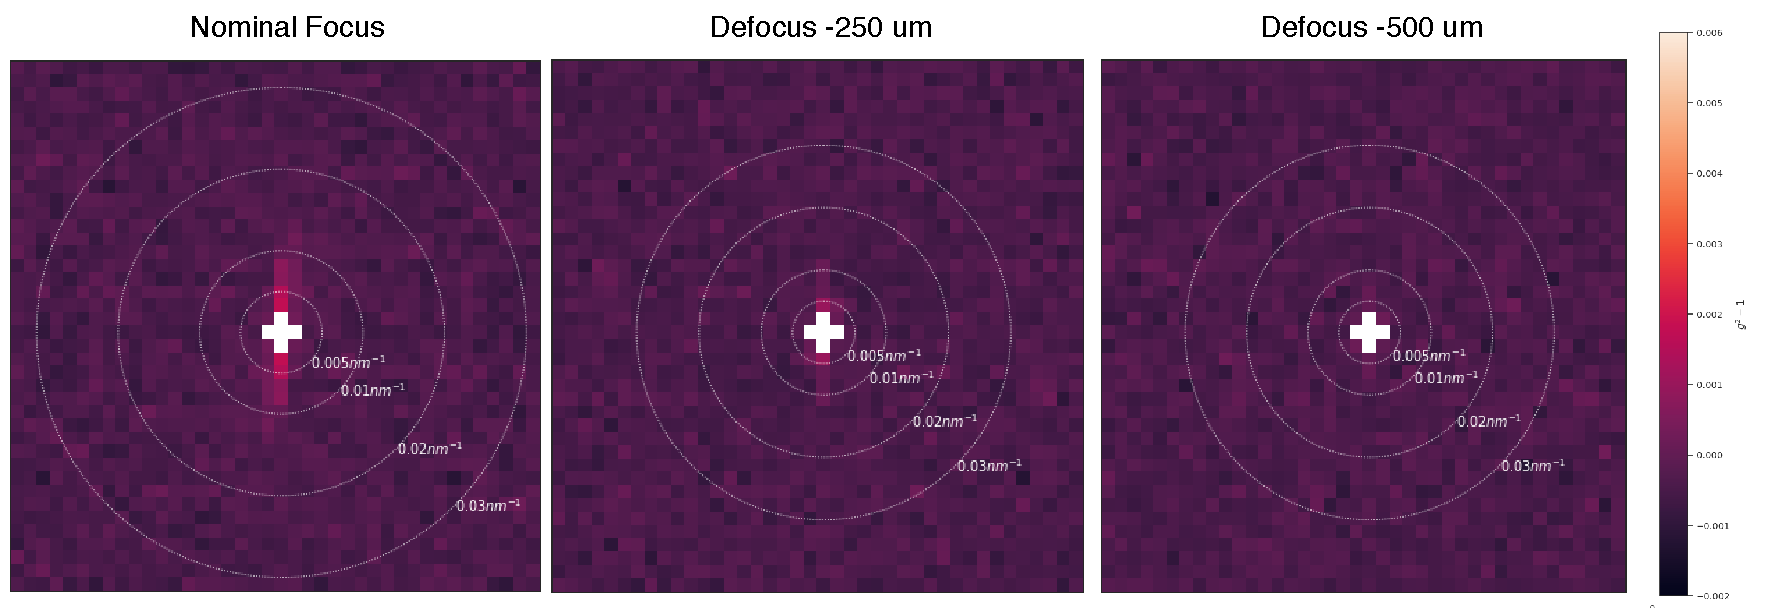
\includegraphics[width=0.9\linewidth]{images/Cu5um_reco2d.pdf}
	\caption[Results copper foil]{Results of the $g^2-1$ calculation for the 5\,\textmu m copper foil placed at the focus as well as at two positions outside the focus (along the X-ray beam). As the focal width increases due to the defocusing, its extent in the reconstructed reciprocal space decreases until at -500\,\textmu m defocus it can no longer be reconstructed. The narrow extent in horizontal direction in reciprocal spaces causes undersampling and contrast reduction. }
	\label{fig:Cu5umreco2d}
\end{figure}
\begin{figure}
	\centering
	\begin{subfigure}[b]{0.9\textwidth}
		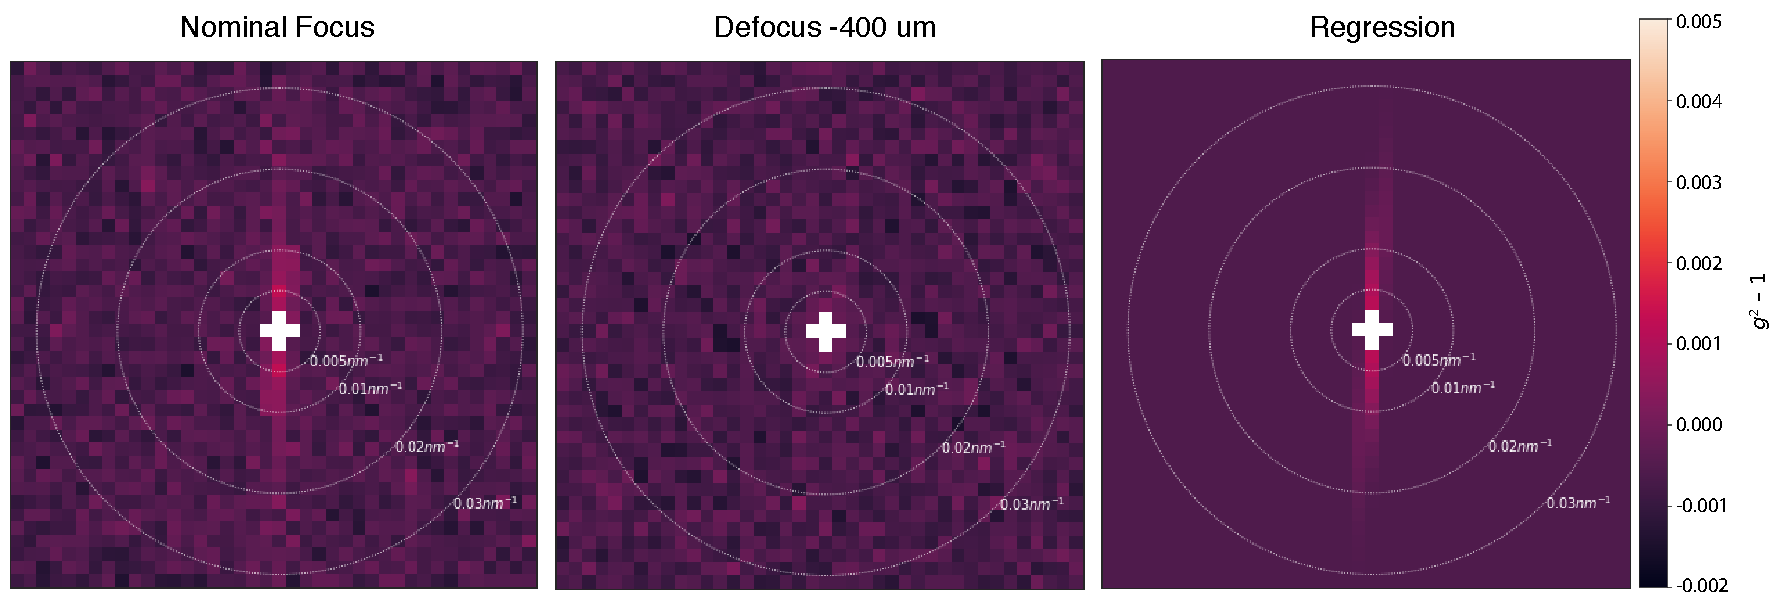
\includegraphics[width=\linewidth]{images/Fe10um_reco2d.pdf}
		\caption{10\,\textmu m iron foil}
		\label{fig:fe10umreco2d}
	\end{subfigure}
	\begin{subfigure}[b]{0.9\textwidth}
		\includegraphics[width=\linewidth]{images/Fe500nm_reco2d.pdf}
		\caption{500\,nm iron foil}
		\label{fig:fe500nmreco2d}
	\end{subfigure}
	\caption[Results iron foils]{\textbf{(a)} $g^2-1$ results for the 10\,\textmu m iron foil placed at the focus as well as outside the focus (along the X-ray beam) and the result obtained by regression on the nominal focus data with fixed true horizontal dimension. This is used to extrapolate the peak amplitude in the masked areas. \textbf{(b)} $g^2-1$ results for the 500\,nm Iron foil at focus as well as at two defocused positions. The SNR is low and the signal almost indistinguishable from noise, but the horizontal extent in reciprocal space is as expected larger. Due to the low SNR no reliable regression of the focal size can be performed.}
	\label{fig:fereco2d}
\end{figure}
\begin{figure}
	\centering
	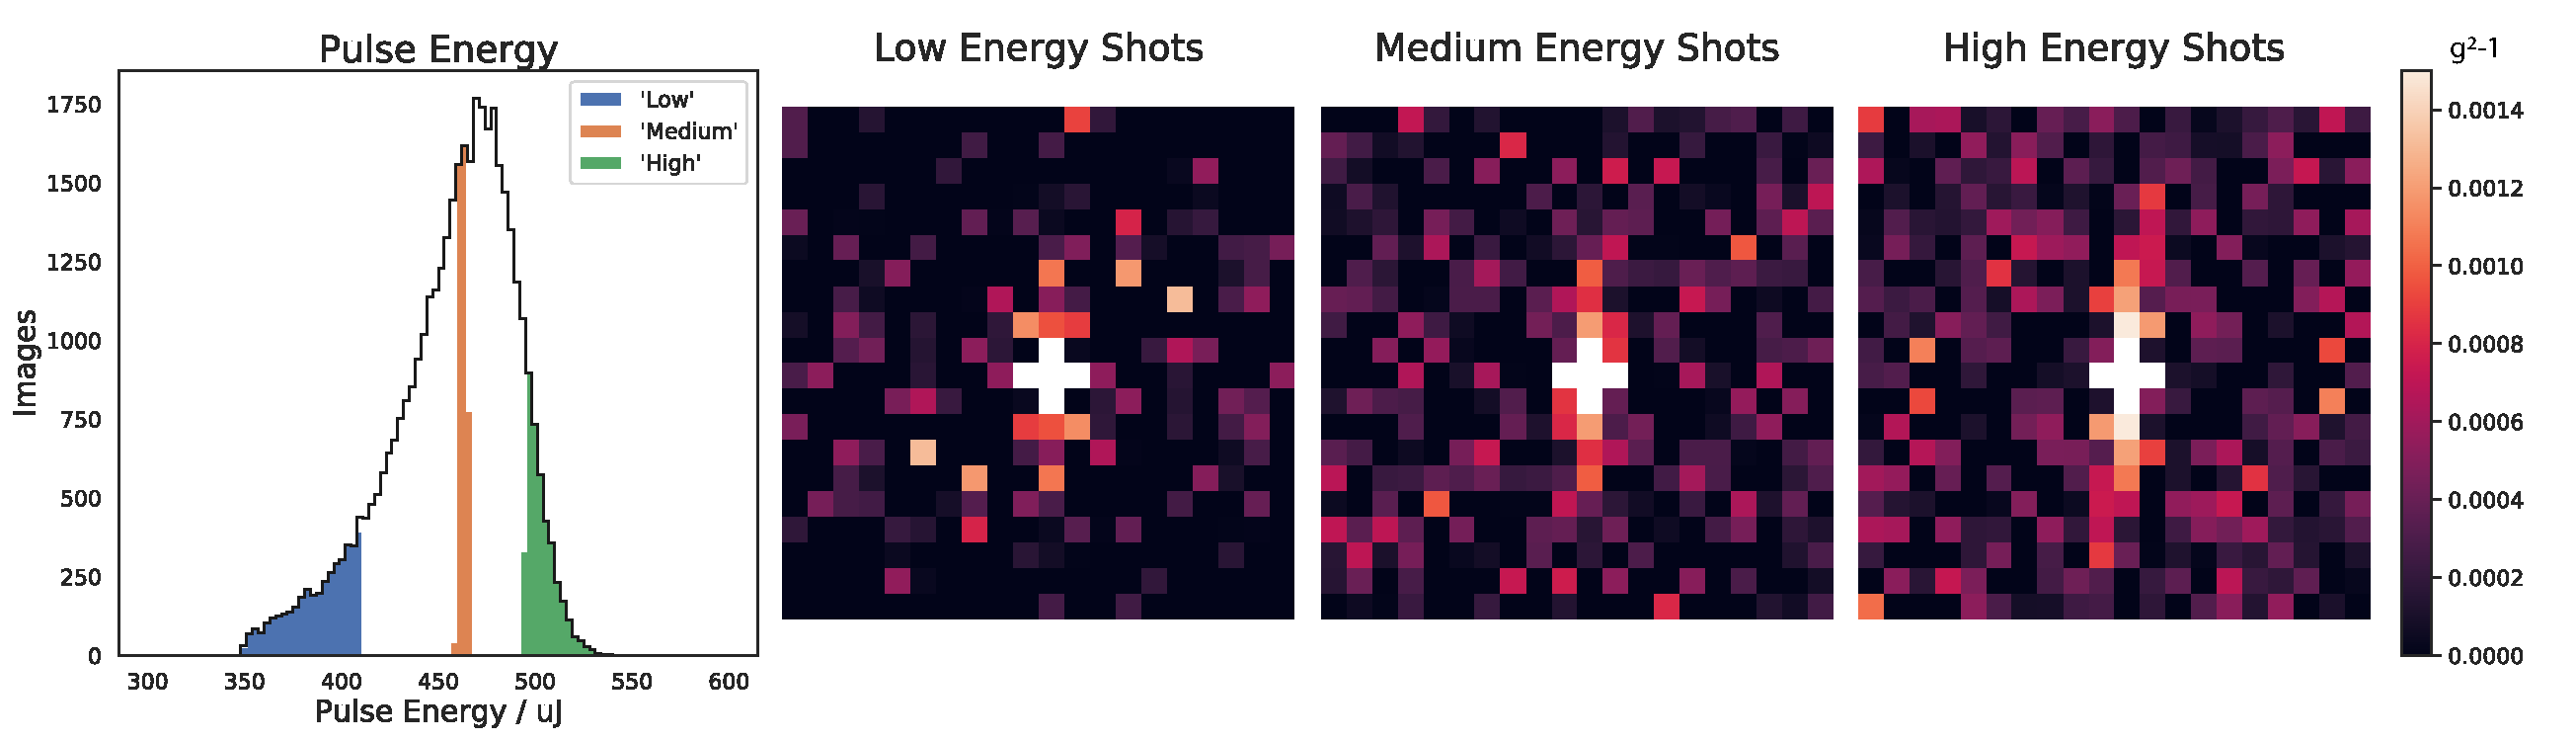
\includegraphics[width=\linewidth]{images/energy_binned.pdf}
	\caption[Excitation energy binned reconstruction]{$g^2-1$ results using a 5\,\textmu m copper foil placed at the focus as the sample. The reconstructions have been performed on 4000 images each (see histogram on the left)  selected by excitation pulse energy estimates by upstream energy detectors as surrogate for the pulse length, similar to the data selection in previous experiments at SACLA \cite{inoue2019}. Regression of the signal amplitude as (as described in the main text) shows a slight difference: 0.0038$\pm$0.0007 for the low energy shots, 0.0043$\pm$0.0007 for the medium energy shots and 0.0052$\pm$0.0007 for the high energy shots. This confirms the validity of dropping low energy shots from the reconstruction to improve the SNR.}
	\label{fig:energy_binned}
\end{figure}

\subsection{Imaging Nanoparticles}

\begin{figure}
	\centering
	\begin{subfigure}[b]{0.8\textwidth}
		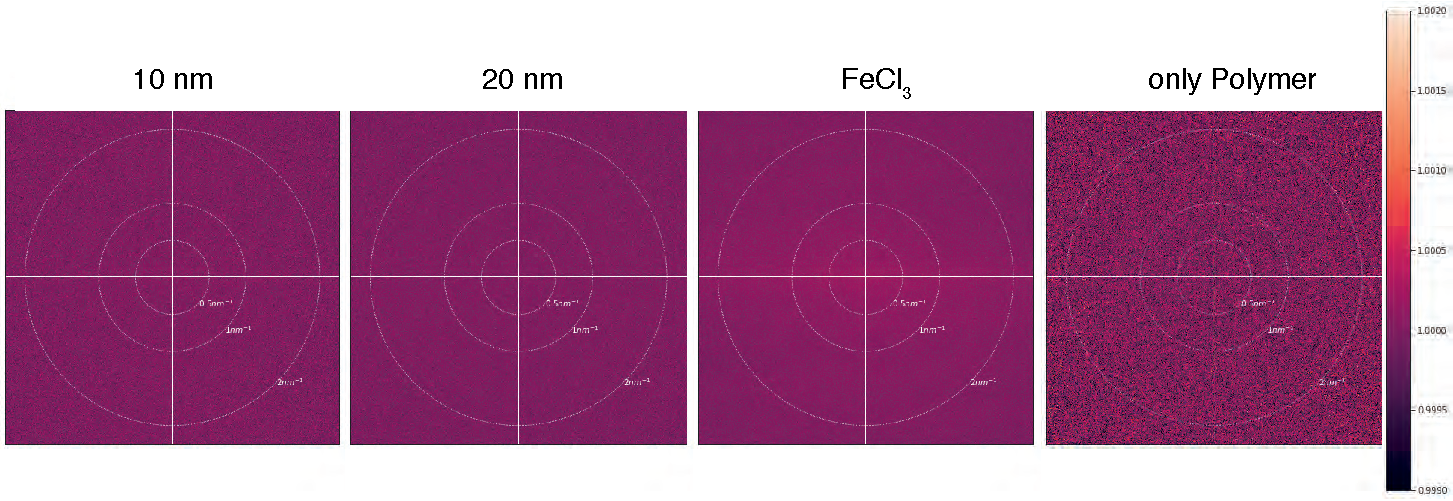
\includegraphics[width=\linewidth]{images/resultnano2dr.pdf}
		\caption{Calculated $g^2$ images of for two nanoparticle samples and two reference samples.}
		\label{fig:resnano2d}
	\end{subfigure}
	\begin{subfigure}[b]{\textwidth}
		\begin{subfigure}[b]{0.49\textwidth}
		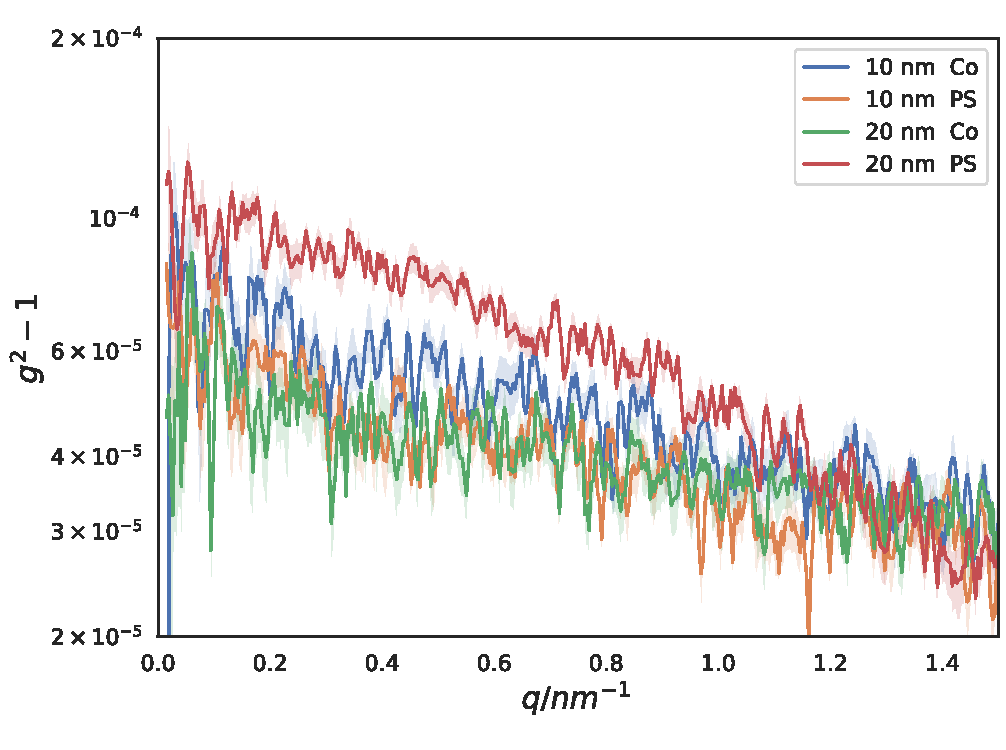
\includegraphics[width=\linewidth]{images/nano.pdf}
		\end{subfigure}
		\begin{subfigure}[b]{0.49\textwidth}
		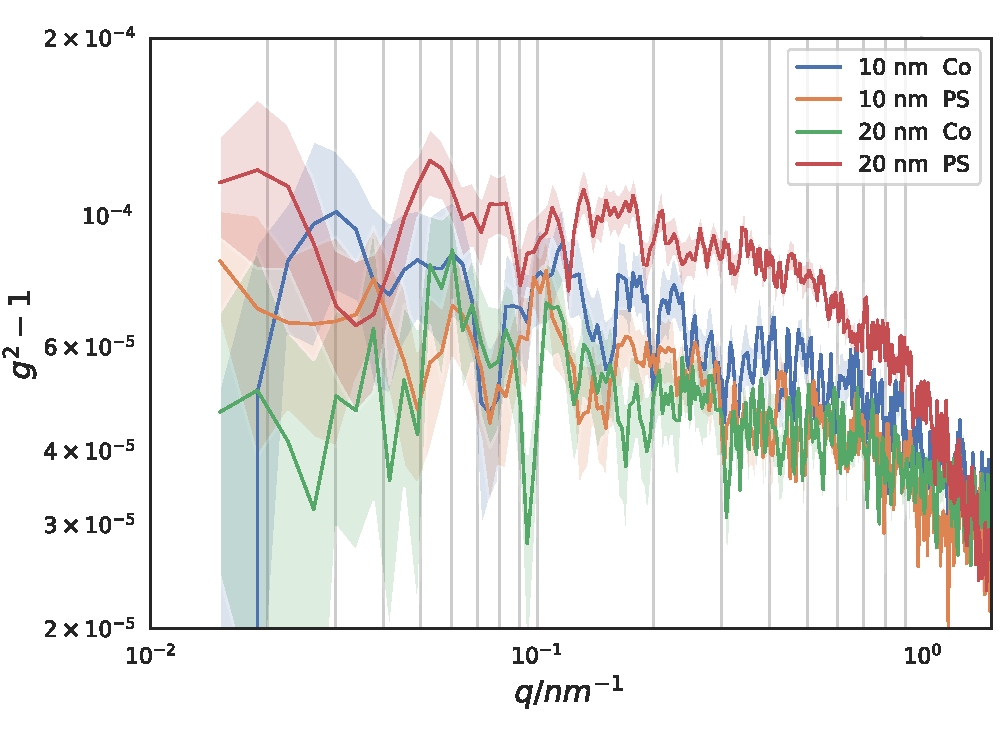
\includegraphics[width=\linewidth]{images/nano_loglog.pdf}
	\end{subfigure}
			\caption{Radial profiles of $g^2$ for different nanoparticle samples.}
			\end{subfigure}
	\label{fig:resnanorad}
	\caption[Results nanoparticles]{\textbf{(a)} 2d images of the calculated $g^2$ of fluorescence patterns recorded on the octal detector of two nanoparticle-in-copolymer samples with 10\,nm and 20\,nm nominal diameter in comparison to two different baseline samples, (mostly homogeneous in the polymer distributed) iron chloride and the polymer matrix without any added iron. The detector artifacts are almost completely removed in those images. \textbf{(b)} Radial profiles of the calculated $g^2$ of two differently sized nanoparticles in the two different polymer matrices after applying a linear Savitzky-Golay filter (window 3 pixel $\overset{\scriptscriptstyle\wedge}{=}$ 0.02\,nm$^{-1}$). The color bands denote the standard error of the radial mean. None of the expected features are clearly visible in the reconstruction. }
	\label{fig:resnano}
\end{figure}

The mean number of counted signal photons per pixel after filtering is $0.03\pm0.01$ for the nanoparticle samples as well as the iron chloride reference sample, the number of images analyzed has been limited to 30,000 for each sample, with the exception of the \enquote{10\,nm in PS} sample only having 25,000 usable shots after filtering. At similar signal photon counts on the octal as observed for the foils on the dual detector, the peak in the spectrum at the energy of the FEL beam is more pronounced, leading to difficulties distinguishing higher numbers of photons. Hence, only one and two photon hits are used in the photon discretization (see \fref{fig:spectrum_nano} for an example).

Using a sample with just the polymer, without any added iron (neither nanoparticles nor atomic), the influence of air scattering on the correlations can be examined, and in the results of the iron chloride sample having similar numbers of signal photons the effect of uncorrected detector artifacts could be seen. Neither result in a strong correlation signal (see \fref{fig:resnano2d}). The strength of the noise as quantified by the standard deviation over pixels outside the center area of the 2d-reconstruction of the samples is (1.4$\pm$0.1)$\cdot$10$^{-4}$.

In the radially averaged $g^2$ of the four different samples neither a feature corresponding to the distance of aggregated particles (as visible in the SAXS measurements)  nor a minimum at $q\approx4.5/r$, indicative of spherical samples, can be distinguished. 
\FloatBarrier
\subsection{Imaging Crystals}

After applying the filtering, masking and corrections, the mean photon count considered as signal per pixel is 0.4-0.6 for both samples (a histogram is shown in \fref{fig:spectrum_gaas}), corresponding to $\approx 3\cdot10^7$ photons in $4\pi$ and $\approx$1\% of the gallium atoms inside the focus emitting fluorescence. Overall, $2\cdot10^4$ images per sample remain and can be used for further analysis.

For the determination of the crystal orientation and detector offsets, the regression parameters are initialized with a 5.65\,\AA\, lattice constant, 9.25\,keV energy, 14\,cm detector distance and the result of a 2D cubic fit to the fluorescence background for the values of the x- and y-shifts. The  lines considered are shown in \fref{fig:kosselgaaslines} and listed in \fref{tab:kosselpeaks}. The results are shown in \fref{tab:kosselfit} as mean over the sets for each sample and maximum deviation from the mean as an error estimation. Overall, the alignment is precise up to at most than 0.6° rotation, except for rotation in the plane parallel to the crystal surface (designated \textit{roll}), and 140\,pixel translation.

\begin{figure}
	\centering
	\begin{subfigure}{0.35\textwidth}
		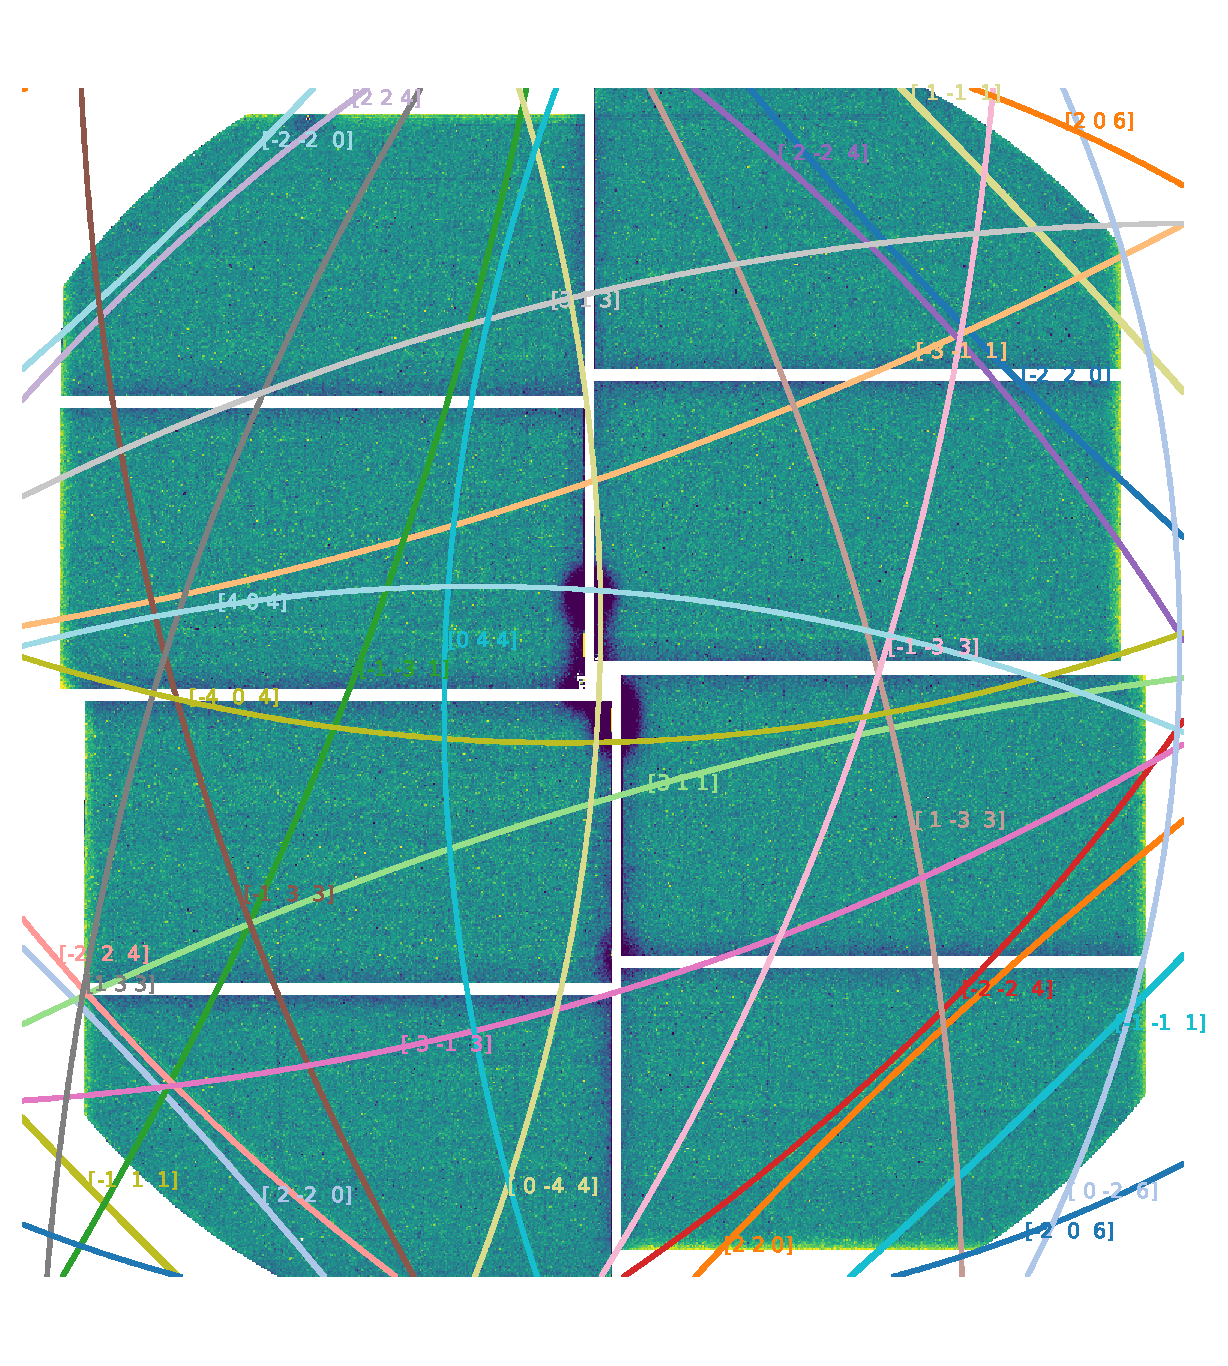
\includegraphics[width=\linewidth]{images/kossel_gaas1r.pdf}
		\caption{Indexed lines on sample 1}
	\end{subfigure}
	\hspace{0.2cm}
	\begin{subfigure}{0.35\textwidth}
		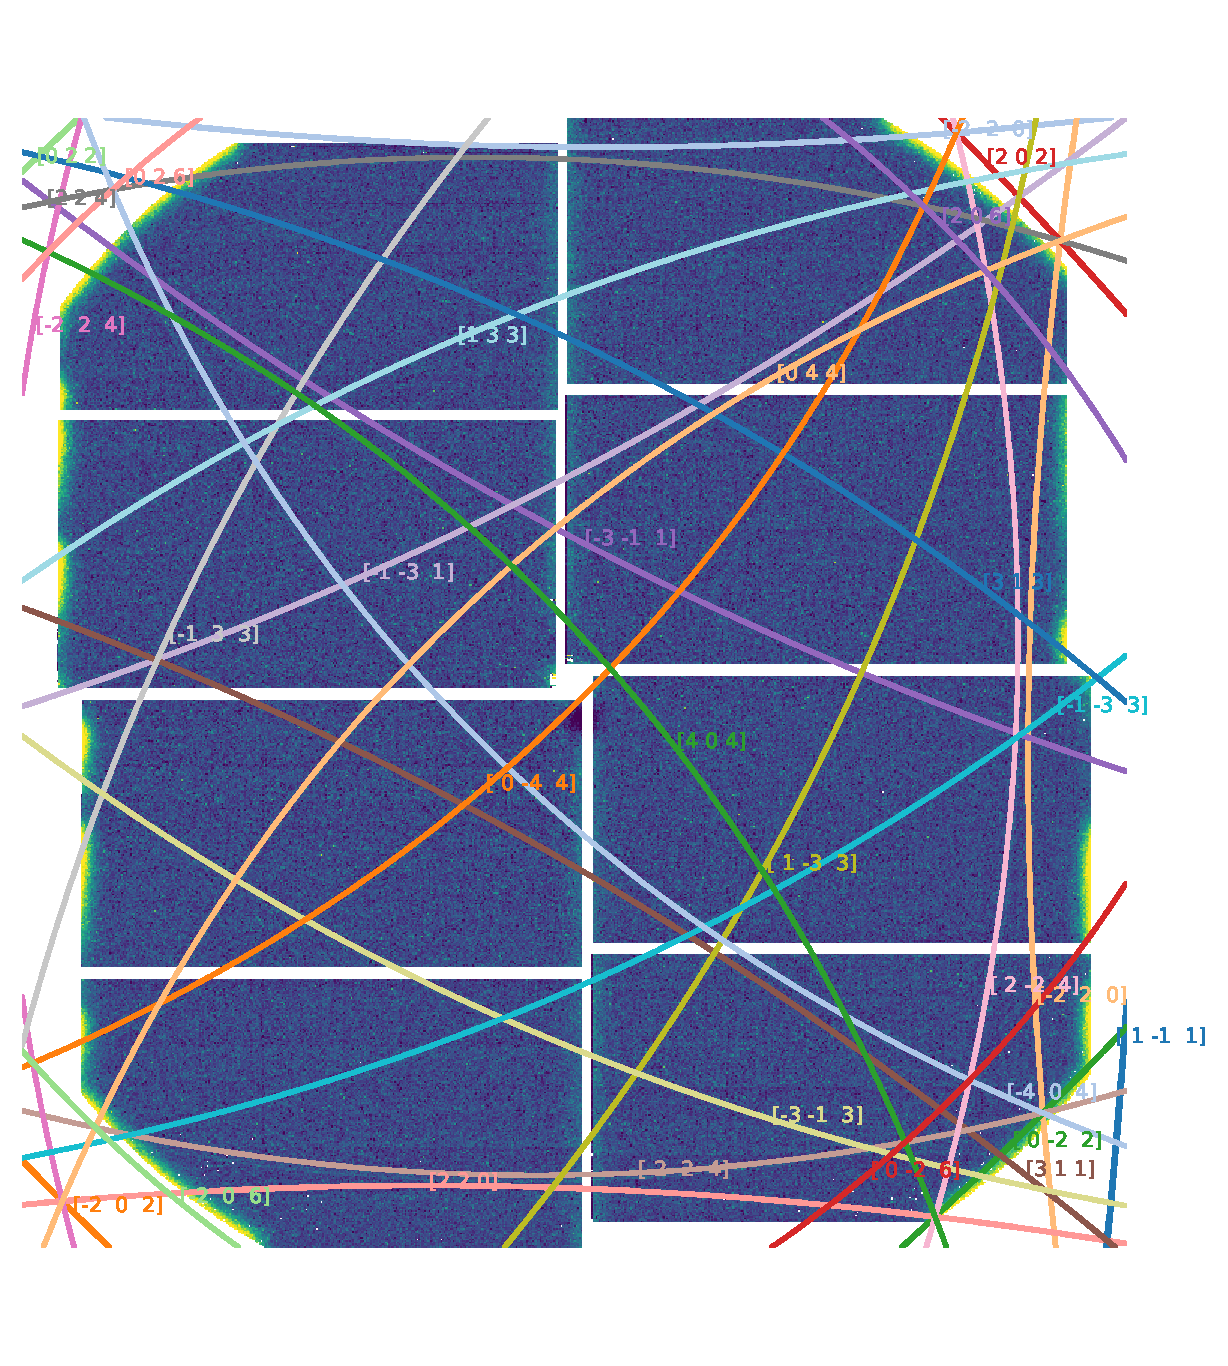
\includegraphics[width=\linewidth]{images/kossel_gaas2r.pdf}
		\caption{Indexed lines on sample 2}
	\end{subfigure}
	\caption[Kossel lines on GaAs samples]{Indexed Kossel lines in the determined orientation overlaid over the mean of 5000 shots after background subtraction. For a list of all considered indices, see  \fref{tab:kosselpeaks}.}
	\label{fig:kosselgaaslines}
\end{figure}

\begin{table}[]
	\caption{Results of the Kossel line analysis}
	\begin{small}
		\begin{tabular}{llllllll}
			\hline
			Sample & \multicolumn{2}{l}{Offset of Detector} & \multicolumn{3}{l}{Rotation of Detector}  & Detector Distance &  \\
			& x in mm        & y in mm        & yaw              & pitch           & roll           & in mm             &  \\ 
			\hline
			GaAs 1 & 1.4$\pm$0.2    & 6.4$\pm$0.4    & -0.4°$\pm$0.2° & 0.1°$\pm$0.2° & 1.5°$\pm$0.2° & 141.7$\pm$0.8     &  \\
			GaAs 2 & 1.3$\pm$0.2    & 5.8$\pm$0.3    & -0.2°$\pm$0.3° & 0.1°$\pm$0.2° & 46.1°$\pm$0.1° & 139.9$\pm$0.8     &  \\
			\hline
		\end{tabular}
	\end{small}	
	\label{tab:kosselfit}
\end{table}

Using the determined rotation and translation to determine for each pixel the corresponding $\vec{q}$ and performing the corrected reconstruction (averaging over all images left after filtering) results in a volume of 3750\,x\,4032\,x\,500 pixels$^3$ with maximum extent of approx. $\pm$3\,x\,$\pm$3\,x\,0.5 \AA$^{-3}$. The non-trivial shape of the reconstructed volume is influenced by the the placement of the 8 individual tiles of the detector, the applied mask to each tile as well as the overall detector offset and slight rotation.

 In slices in the $q_z=$\,0\,nm$^{-1}$ plane, Bragg peaks with an Laue index $h=0$ should be visible. As the determined detector rotation has an estimated uncertainty of approximately $\pm$0.2° in each direction, maximum intensity projections along 10 $q_z$ slices (up to $q_z\approx$\,0.15\,nm$^{-1}$) are shown in \fref{fig:resgaas1} to ensure Bragg peaks slightly rotated out the of the plane would still be visible. Marked areas in the overview on the left are shown in detail on the right. The noise level in the regions of interest around the expected Bragg peak positions (estimated from the standard deviation over all pixels in the regions) is 0.0002$\pm$0.0001.  No Bragg peaks are clearly distinguishable, i.e. higher than 4$\sigma$,  in the result. Similar results for the 45° rotated second sample are shown in \fref{fig:resgaas2}. In both results, the noise level increases in areas with fewer pairs of pixels of the masked detector image contributing, areas with less than 100 pairs are masked and not shown.
 
 \begin{figure}
\begin{subfigure}[b]{\textwidth}
	\centering
	\begin{subfigure}[b]{0.55\textwidth}
		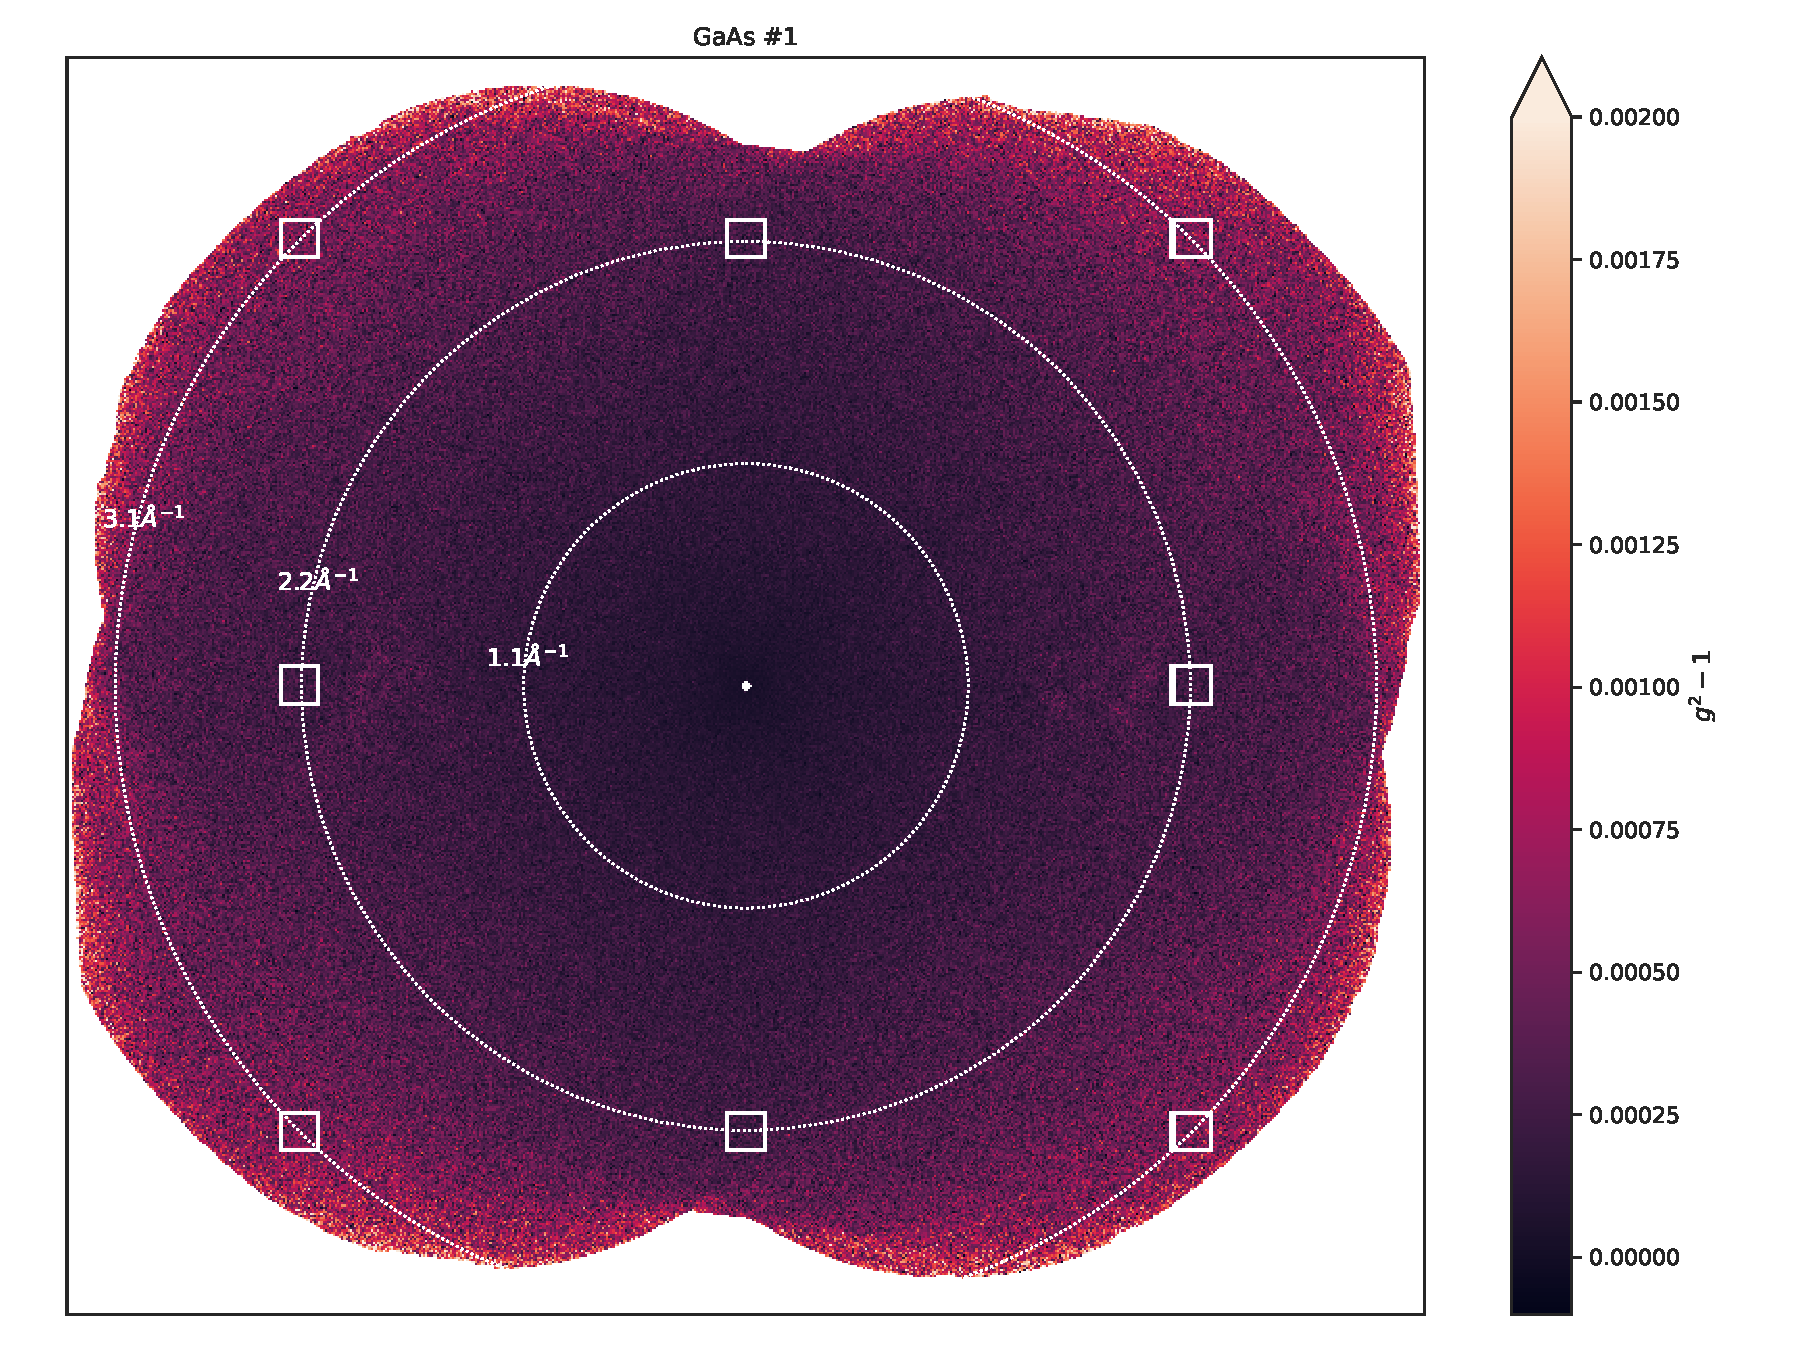
\includegraphics[width=\linewidth]{images/gaas1_overview.pdf}
	\end{subfigure}
	\begin{subfigure}[b]{0.4\textwidth}
		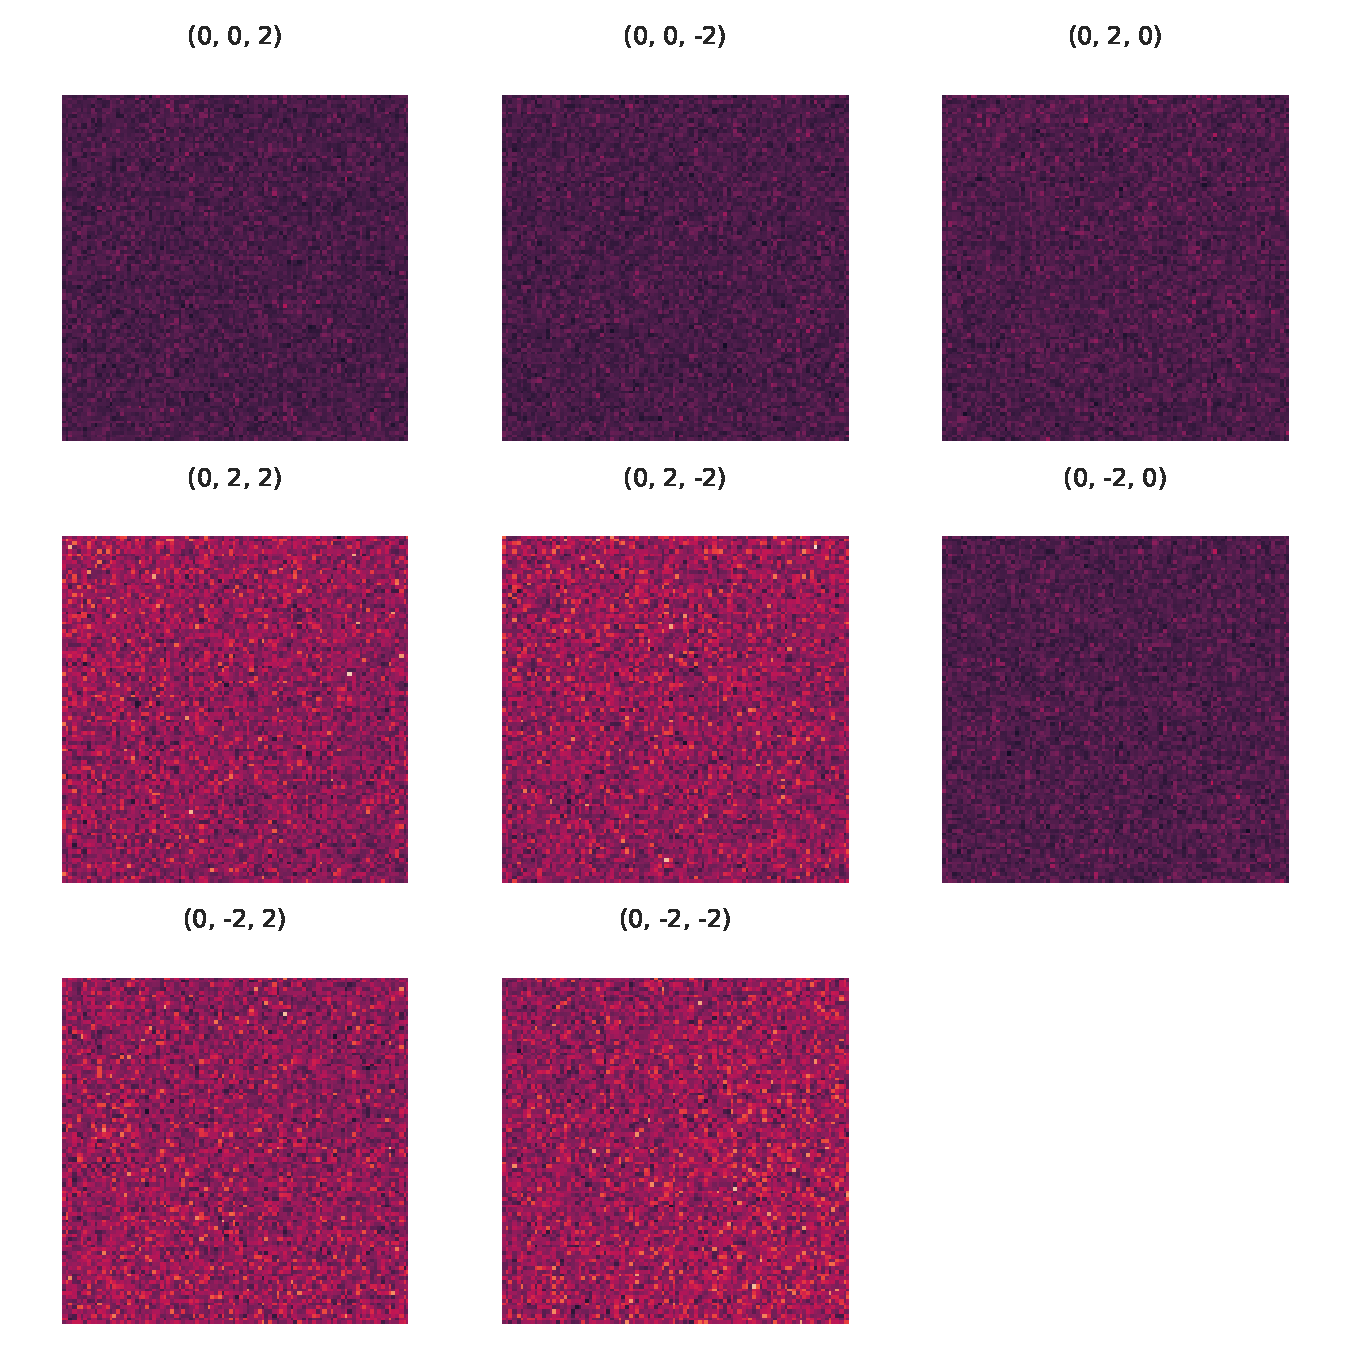
\includegraphics[width=\linewidth]{images/gaas1_zoom.pdf}
	\end{subfigure}
	\caption[Results GaAs Sample 1]{GaAs sample 1}
	\label{fig:resgaas1}
\end{subfigure}
\begin{subfigure}[b]{\textwidth}
	\centering
	\begin{subfigure}[b]{0.55\textwidth}
		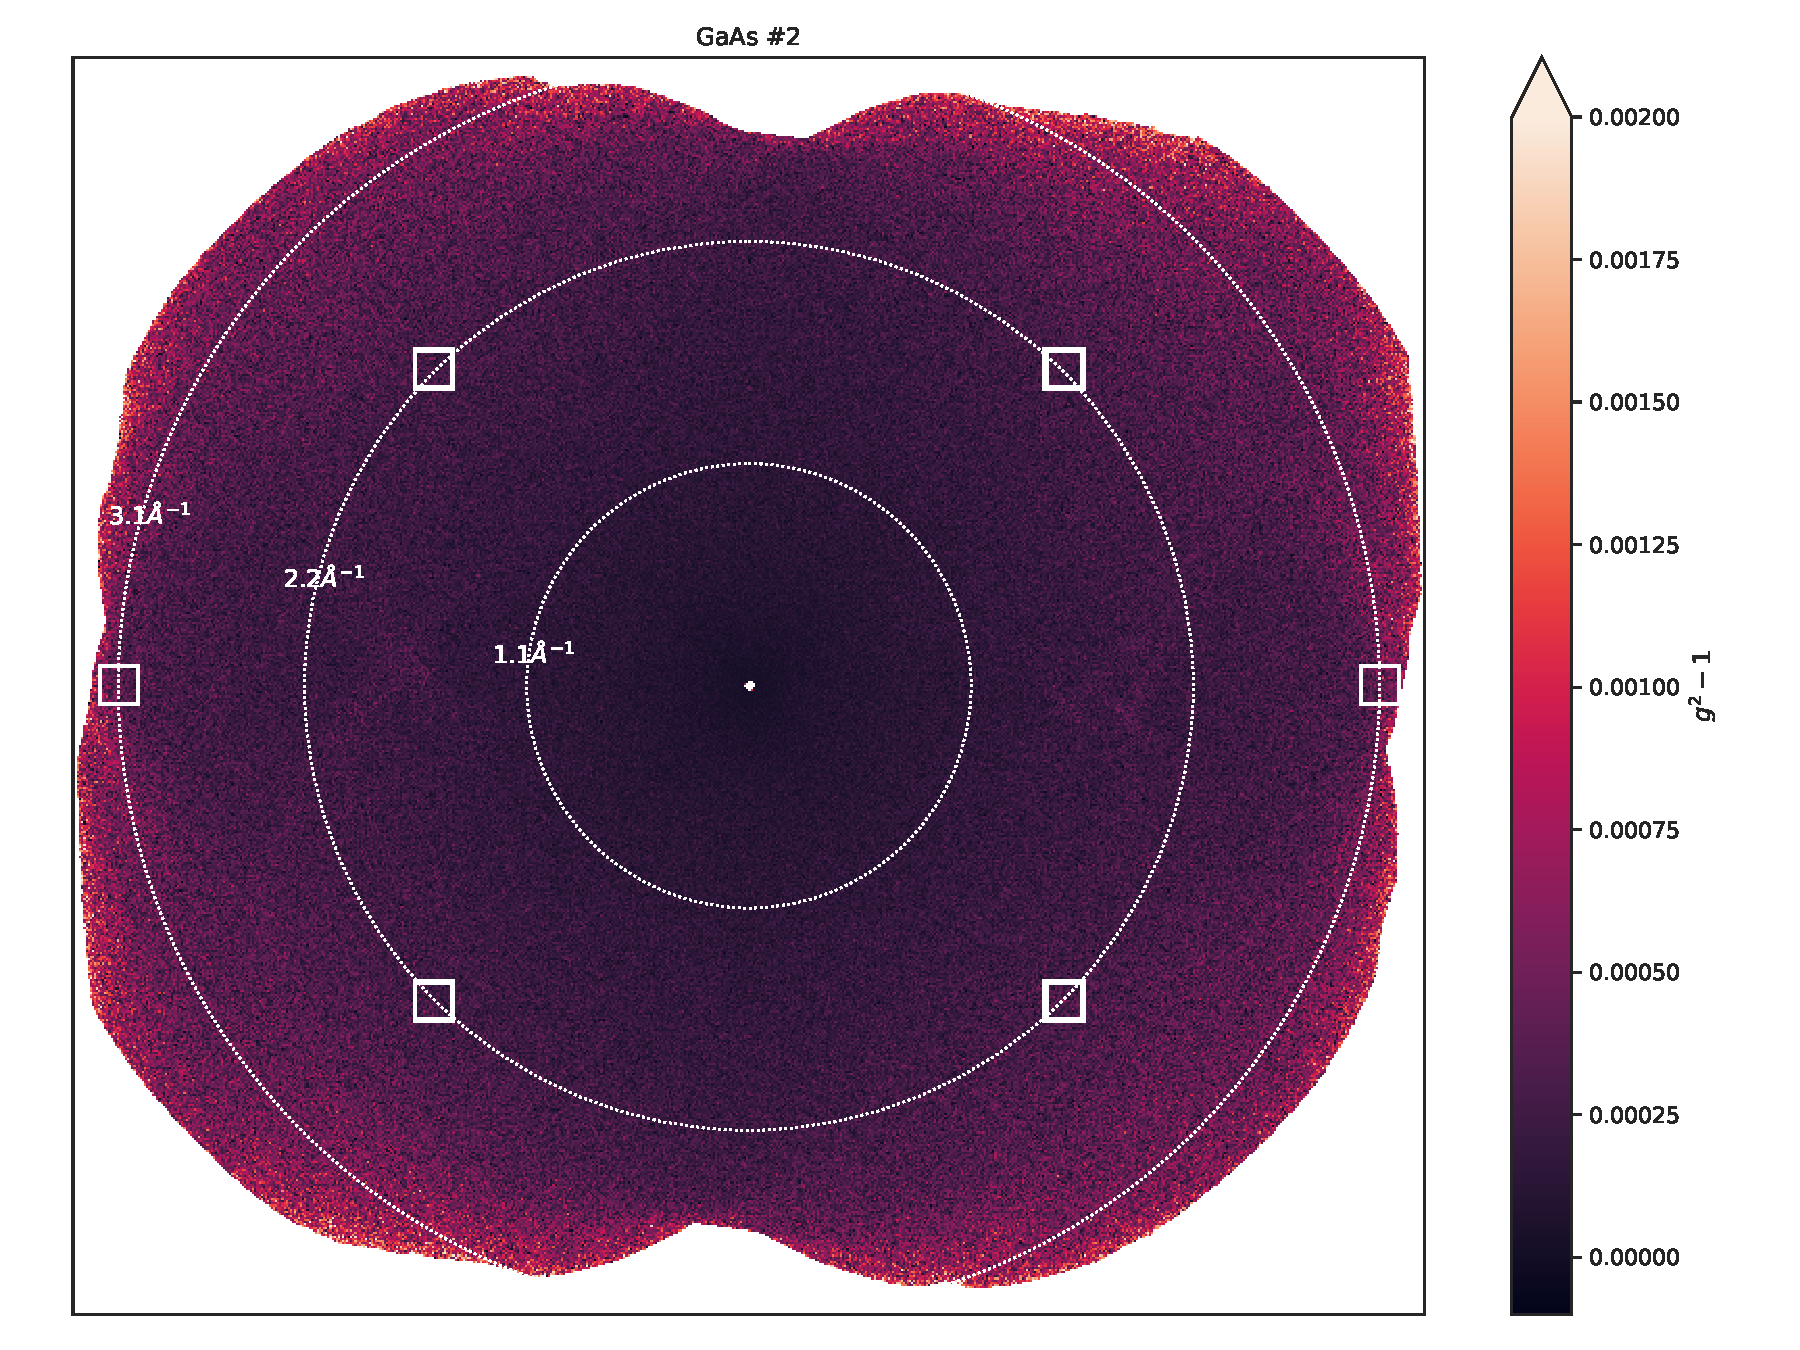
\includegraphics[width=\linewidth]{images/gaas2_overview.pdf}
	\end{subfigure}
	\begin{subfigure}[b]{0.4\textwidth}
		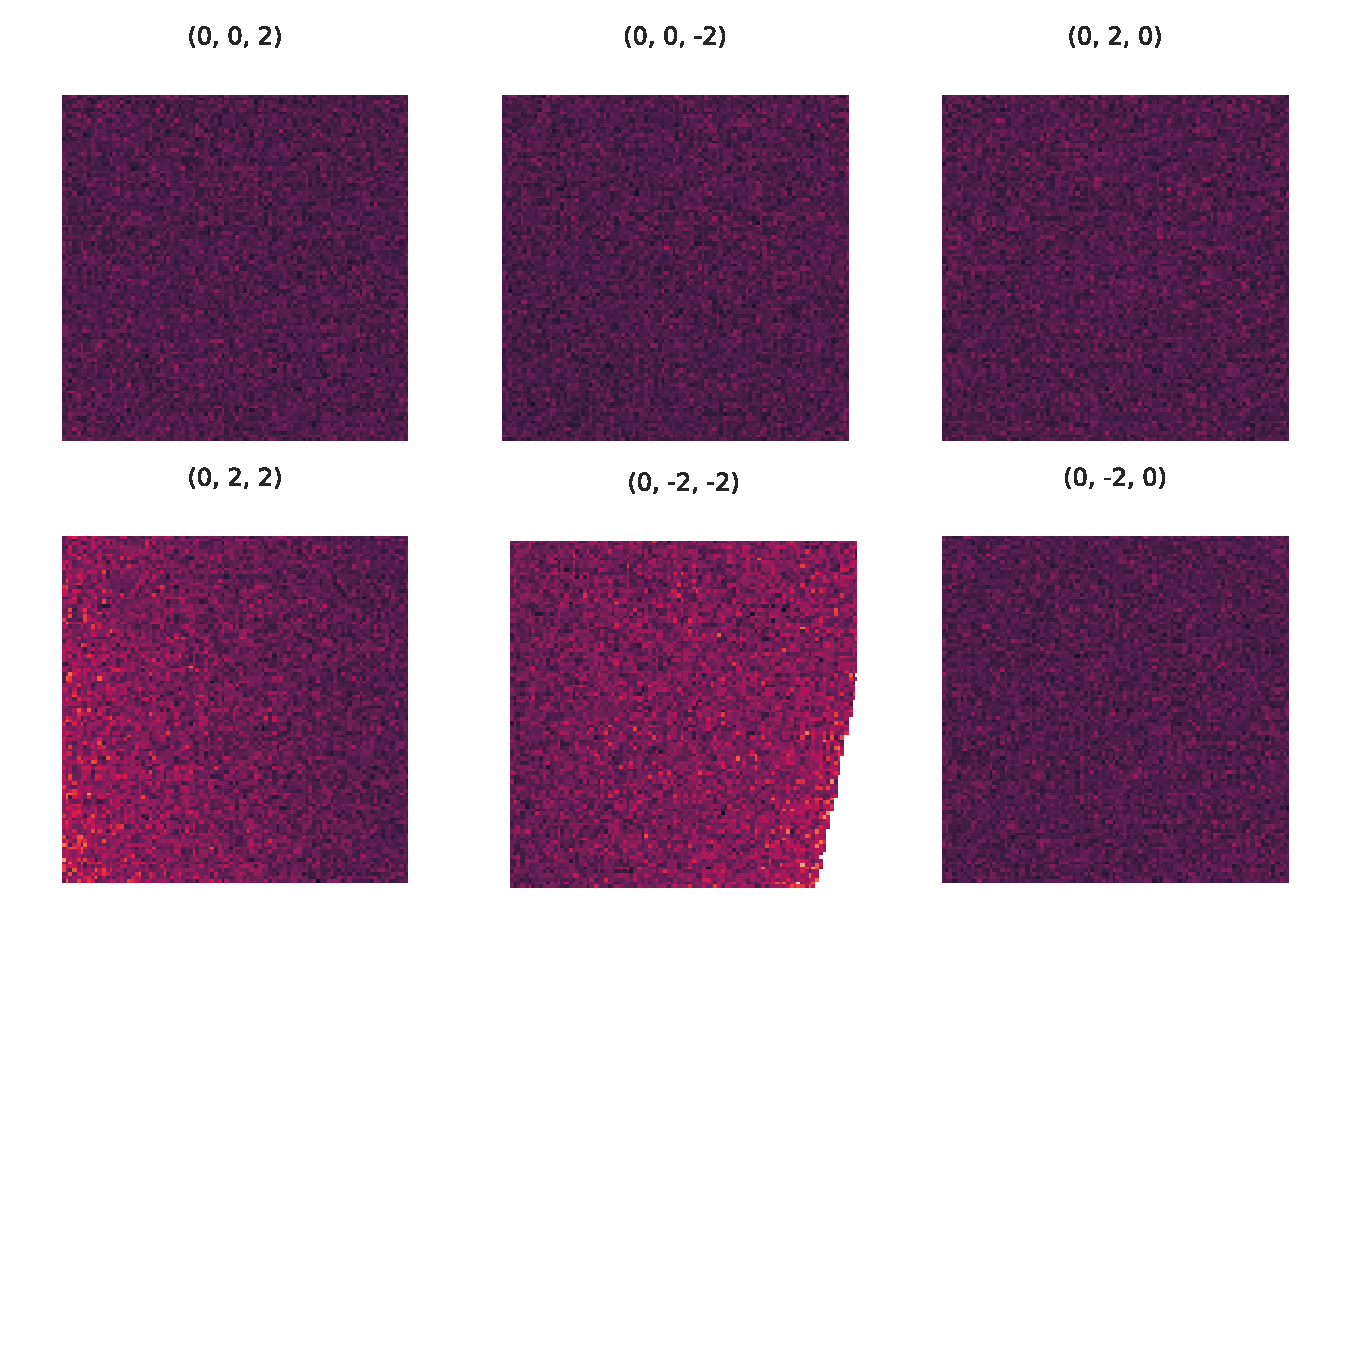
\includegraphics[width=\linewidth]{images/gaas2_zoom.pdf}
	\end{subfigure}
	\caption[Results GaAs Sample 2]{Gaas sample 2}
	\label{fig:resgaas2}
\end{subfigure}
	\caption[Results GaAs Samples]{Result of the $g^2$  calculation for the GaAs single crystal samples.  MIP from $q_z$=0\,nm$^{-1}$ to 0.3\,nm$^{-1}$. Marked areas in the overview on the left around expected positions of Bragg peaks are shown in detail on the right (labeled by the corresponding Laue indices). The crystal in sample 2 is 45° rotated compared to sample 1, leading to less Bragg positions being inside the reconstructed plane. No Bragg peaks are  clearly distinguishable in the result.}
 \end{figure}
